% -*- Mode:TeX -*-

%% IMPORTANT: The official thesis specifications are available at:
%%            http://libraries.mit.edu/archives/thesis-specs/
%%
%%            Please verify your thesis' formatting and copyright
%%            assignment before submission. If you notice any
%%            discrepancies between these templates and the
%%            MIT Libraries' specs, please let us know
%%            by e-mailing thesis@mit.edu


%% The documentclass options along with the pagestyle can be used to generate
%% a technical report, a draft copy, or a regular thesis. You may need to
%% re-specify the pagestyle after you \include cover.tex. For more
%% information, see the first few lines of mitthesis.cls.

%\documentclass[12pt,vi,twoside]{mitthesis}
%%
%%  If you want your thesis copyright to you instead of MIT, use the
%%  ``vi'' option, as above.
%%
%\documentclass[12pt,twoside,leftblank]{mitthesis}
%%
%% If you want blank pages before new chapters to be labelled ``This
%% Page Intentionally Left Blank'', use the ``leftblank'' option, as
%% above.

\documentclass[12pt,twoside]{mitthesis}
\usepackage{lgrind}
%% These have been added at the request of the MIT Libraries, because
%% some PDF conversions mess up the ligatures.  -LB, 1/22/2014
\usepackage{cmap}
\usepackage{verbatim}
\usepackage{amsmath}
\usepackage{booktabs}
\usepackage{graphicx}
\usepackage{array}
\usepackage{float}
\usepackage{ragged2e}
\usepackage{adjustbox}
\usepackage{caption}
\usepackage[T1]{fontenc}
\pagestyle{plain}
\graphicspath{{C:/repos/learn-doing/thesis/figures/}{C:/repos/learn-doing/R/Output/}}
%% This bit allows you to either specify only the files which you wish to
%% process, or `all' to process all files which you \include.
%% Krishna Sethuraman (1990).

%\typein [\files]{Enter file names to process, (chap1,chap2 ...), or `all' to process all files:}
\def\all{all}
\ifx\files\all \typeout{Including all files.} \else %\typeout{Including only \files.} \includeonly{\files} \fi

\begin{document}

%% -*-latex-*-
%
% For questions, comments, concerns or complaints:
% thesis@mit.edu
%
%
% $Log: cover.tex,v $
% Revision 1.9  2019/08/06 14:18:15  cmalin
% Replaced sample content with non-specific text.
%
% Revision 1.8  2008/05/13 15:02:15  jdreed
% Degree month is June, not May.  Added note about prevdegrees.
% Arthur Smith's title updated
%
% Revision 1.7  2001/02/08 18:53:16  boojum
% changed some \newpages to \cleardoublepages
%
% Revision 1.6  1999/10/21 14:49:31  boojum
% changed comment referring to documentstyle
%
% Revision 1.5  1999/10/21 14:39:04  boojum
% *** empty log message ***
%
% Revision 1.4  1997/04/18  17:54:10  othomas
% added page numbers on abstract and cover, and made 1 abstract
% page the default rather than 2.  (anne hunter tells me this
% is the new institute standard.)
%
% Revision 1.4  1997/04/18  17:54:10  othomas
% added page numbers on abstract and cover, and made 1 abstract
% page the default rather than 2.  (anne hunter tells me this
% is the new institute standard.)
%
% Revision 1.3  93/05/17  17:06:29  starflt
% Added acknowledgements section (suggested by tompalka)
%
% Revision 1.2  92/04/22  13:13:13  epeisach
% Fixes for 1991 course 6 requirements
% Phrase "and to grant others the right to do so" has been added to
% permission clause
% Second copy of abstract is not counted as separate pages so numbering works
% out
%
% Revision 1.1  92/04/22  13:08:20  epeisach

% NOTE:
% These templates make an effort to conform to the MIT Thesis specifications,
% however the specifications can change. We recommend that you verify the
% layout of your title page with your thesis advisor and/or the MIT
% Libraries before printing your final copy.
\title{Master of Arts Thesis}

\author{Maximiliano  Gonzalez}
% If you wish to list your previous degrees on the cover page, use the
% previous degrees command:
%       \prevdegrees{A.A., Harvard University (1985)}
% You can use the \\ command to list multiple previous degrees
%       \prevdegrees{B.S., University of California (1978) \\
%                    S.M., Massachusetts Institute of Technology (1981)}
\department{Kenneth C. Griffin Department of Economics}

% If the thesis is for two degrees simultaneously, list them both
% separated by \and like this:
% \degree{Doctor of Philosophy \and Master of Science}
\degree{Master of Arts in Social Sciences, Economics Concentration}

% As of the 2007-08 academic year, valid degree months are September,
% February, or June.  The default is June.
\degreemonth{April}
\degreeyear{2021}
\thesisdate{April 18, 2021}

%% By default, the thesis will be copyrighted to MIT.  If you need to copyright
%% the thesis to yourself, just specify the `vi' documentclass option.  If for
%% some reason you want to exactly specify the copyright notice text, you can
%% use the \copyrightnoticetext command.
%\copyrightnoticetext{\copyright IBM, 1990.  Do not open till Xmas.}

% If there is more than one supervisor, use the \supervisor command
% once for each.
\supervisor{William J. Supervisor}{Associate Professor}

% This is the department committee chairman, not the thesis committee
% chairman.  You should replace this with your Department's Committee
% Chairman.
\chairman{Arthur C. Chairman}{Chairman, Department Committee on Graduate Theses}

% Make the titlepage based on the above information.  If you need
% something special and can't use the standard form, you can specify
% the exact text of the titlepage yourself.  Put it in a titlepage
% environment and leave blank lines where you want vertical space.
% The spaces will be adjusted to fill the entire page.  The dotted
% lines for the signatures are made with the \signature command.
\maketitle

% The abstractpage environment sets up everything on the page except
% the text itself.  The title and other header material are put at the

% top of the page, and the supervisors are listed at the bottom.  A
% new page is begun both before and after.  Of course, an abstract may
% be more than one page itself.  If you need more control over the
% format of the page, you can use the abstract environment, which puts
% the word "Abstract" at the beginning and single spaces its text.

%% You can either \input (*not* \include) your abstract file, or you can put
%% the text of the abstract directly between the \begin{abstractpage} and
%% \end{abstractpage} commands.

% First copy: start a new page, and save the page number.
\cleardoublepage
% Uncomment the next line if you do NOT want a page number on your
% abstract and acknowledgments pages.
% \pagestyle{empty}
\setcounter{savepage}{\thepage}
\begin{abstractpage}


\centering
\textbf{Abstract}
\justify
\footnotesize
Using 43,000 public construction contracts in Chile procured via competitive calls for proposals, I study the effect of firm experience on the likelihood of winning a contract in the future. To address endogeneity of experience (better firms tend to win more contracts in the past and in the future), I instrument firm experience with the number of past contracts won in closely contested auctions, where close auctions are defined as either i) having close monetary bids and price as an important awarding factor, or ii) involving closely ranked firms (via a multiplayer Elo algorithm) . The IV estimates indicate that firm's experience increases the proportion of contracts won by seven percentage points (roughly a third of the winning rate of firms with no experience). I investigate possible mechanisms that could explain this increase in market success by studying improvements along i) cost measures and ii) quality variables. I find that experienced firms submit bids which are three percentage points lower than firms with no experience. Additionally, experienced firms increase in ten percentage points the approval rate of their proposals in the first stage of the awarding process. I discuss the magnitude of the findings and possible implications for public auction design.

\end{abstractpage}

% Additional copy: start a new page, and reset the page number.  This way,
% the second copy of the abstract is not counted as separate pages.
% Uncomment the next 6 lines if you need two copies of the abstract
% page.
% \setcounter{page}{\thesavepage}
% \begin{abstractpage}
% 

\centering
\textbf{Abstract}
\justify
\footnotesize
Using 43,000 public construction contracts in Chile procured via competitive calls for proposals, I study the effect of firm experience on the likelihood of winning a contract in the future. To address endogeneity of experience (better firms tend to win more contracts in the past and in the future), I instrument firm experience with the number of past contracts won in closely contested auctions, where close auctions are defined as either i) having close monetary bids and price as an important awarding factor, or ii) involving closely ranked firms (via a multiplayer Elo algorithm) . The IV estimates indicate that firm's experience increases the proportion of contracts won by seven percentage points (roughly a third of the winning rate of firms with no experience). I investigate possible mechanisms that could explain this increase in market success by studying improvements along i) cost measures and ii) quality variables. I find that experienced firms submit bids which are three percentage points lower than firms with no experience. Additionally, experienced firms increase in ten percentage points the approval rate of their proposals in the first stage of the awarding process. I discuss the magnitude of the findings and possible implications for public auction design.

% \end{abstractpage}

\cleardoublepage

\section*{Acknowledgments}

This is the acknowledgements section. You should replace this with your
own acknowledgements.

%%%%%%%%%%%%%%%%%%%%%%%%%%%%%%%%%%%%%%%%%%%%%%%%%%%%%%%%%%%%%%%%%%%%%%
% -*-latex-*-

% Some departments (e.g. 5) require an additional signature page.  See
% signature.tex for more information and uncomment the following line if
% applicable.
% % -*- Mode:TeX -*-
%
% Some departments (e.g. Chemistry) require an additional cover page
% with signatures of the thesis committee.  Please check with your
% thesis advisor or other appropriate person to determine if such a 
% page is required for your thesis.  
%
% If you choose not to use the "titlepage" environment, a \newpage
% commands, and several \vspace{\fill} commands may be necessary to
% achieve the required spacing.  The \signature command is defined in
% the "mitthesis" class
%
% The following sample appears courtesy of Ben Kaduk <kaduk@mit.edu> and
% was used in his June 2012 doctoral thesis in Chemistry. 

\begin{titlepage}
\begin{large}
This doctoral thesis has been examined by a Committee of the Department
of Chemistry as follows:

\signature{Professor Jianshu Cao}{Chairman, Thesis Committee \\
   Professor of Chemistry}

\signature{Professor Troy Van Voorhis}{Thesis Supervisor \\
   Associate Professor of Chemistry}

\signature{Professor Robert W. Field}{Member, Thesis Committee \\
   Haslam and Dewey Professor of Chemistry}
\end{large}
\end{titlepage}


%\pagestyle{plain}
%% This is an example first chapter.  You should put chapter/appendix that you
%% write into a separate file, and add a line \include{yourfilename} to
%% main.tex, where `yourfilename.tex' is the name of the chapter/appendix file.
%% You can process specific files by typing their names in at the
%% \files=
%% prompt when you run the file main.tex through LaTeX.
\chapter{Experience and Outcomes
}
The purpose of this chapter is to investigate how past experience affect current outcomes in the market for public construction projects. In order to do so, we slice the data in specific points in time and examine how past experience for a firm is related to future outcomes.

 Section 1 outlines the empirical strategy, .

\section{Data}
Recall that our dataset consist in a set of bids submitted by firms in first-price, sealed bid auctions developed by the government in Chile between 2010 and 2020 for construction projects. The source and main characteristics of the dataset employed in the investigation were detailed in the previous section. Now we detail the specifics of the subset employed for the current research question.

 We further filter the dataset in the following way. we only consider contracts with and estimated price above 20.000.000 CLP to exclude extremely simple contracts, and proposals below 10.000.000 CLP as well. We also excluded contracts without an official estimate. We exclude non-single-item proposals. Finally, we exclude contracts with several proposals from a given contractor as we have no clear way of distinguishing which was the last submitted one.

As a result of the previous filtering steps we end with around 43,000 construction contracts, of the original sample of about 74,000 contracts. We excluded around 5\% of the original sample which had no  official estimate(which are excluded), and around 2\% which are not single-item proposals. By far the most important filtering step is excluding contracts with estimated values of less than 20 MM CLP, which excludes around 41\% of the original dataset (around 30,000 contracts). Finally, around a 1,200 contracts had multiple proposals from the same contractor. Note that some of the previous conditions overlapped among them.

We have contracts in our sample which are awarded based on experience. Contracts awarded with experience as an awarding factor are relevant from the point of past experience, but would bias up our estimates if considered in the computation of outrcomes. Table shows how many contracts have experience in their awarding criteria, how many have price and some descriptive statistics of the weight of each one in the sample.

The table shows descriptive statistics for the final sample employed.
\begin{table}[!h]

\caption{Descriptive Statistics}
\centering
\resizebox{\textwidth}{!}{
\begin{tabular}[t]{cccccc}
\toprule
name & N & mean & std & max & min\\
\midrule
Bid (all) & 119000 & 1.73e+10 & 5.8e+12 & 2e+15 & 1e+07\\
Winning Bid & 32200 & 2.27e+08 & 2.54e+09 & 2.47e+11 & 1e+07\\
Difference between 1st bid and 2nd (\%) & 32200 & 0.0638 & 0.0859 & 0.984 & 0\\
Number of Bidders per Contract & 32200 & 3.18 & 2.25 & 23 & 1\\
Year & 32200 & 2020 & 2.89 & 2020 & 2010\\
Offers made by Firm & 13800 & 8.64 & 18.5 & 846 & 1\\
Win prob. by Firm & 13800 & 0.213 & 0.294 & 1 & 0\\
Offers won by Firm & 13800 & 2.33 & 5.66 & 111 & 0\\
\bottomrule
\end{tabular}
}
\vskip 0.5mm
{\raggedright \footnotesize \underline{Note:} The table shows sample summary statistics for the public construction dataset after filtering has been applied (see text). The difference between 1st(winning) and 2nd (runner-up) bid is only avalaible in approx. 70\% od the contracts, with two or more bidders. \par}
\end{table}



\section{Empirical Strategy}
Our empirical strategy consists in a Regression Discontinuity design in which we compare the bidding outcomes of firms with different levels of previous experience in the market. We first present the baseline OLS specification and then discuss endogeneity issues that arise.

Our two main OLS specification are as follows. $S_{it }$ is the share of contracts won in the period of interest, $EXP_{it} $ is the measure of experience of firm $i$ in period $t-1$ or up until $t$(depending on the specification), and $T_t$ are period fixed effect.
\begin{equation}
\label{eqn:olsspec}
S_{it}=\alpha+ \beta EXP^k_{it-1}+T_t+\varepsilon_{it}
\end{equation}


%Our main interest is the difference between the firms with some and the firms with none experience, but we consider also increasing measures of experience.

Our outcome variable $S_{it }$ is the share of contracts won out of the total amount of contracts bid for, in a specific timeframe. That is, if we consider period $t$, then the outcome variable for firm $i$ is $\dfrac{W_{it}}{B_{it}}$ where $B_{it}$ are the bids submitted by firm $i$ on the period $[t,t+\tau]$, $W_{it}$ are the contracts won in period $[t,t+\tau]$ and $\tau$ is a parameter which controls the duration of the periods in which we compute both outcomes. In our initial specification, we consider each $\tau$ to be equal to two years. Employing a proportion of contracts won instead of total contracts has two advantages. First, we implicitly control by the size of the firm. Second, we capture the learning effects which manifest by being able to bid for contracts where less experienced firms do not submit proposals.

We make an important filtering step before computing outcomes, as we only consider contracts for which previous experience is not among the awarding criteria of the contract. This is because including including contracts for which experience is among the awarding criteria would i) render (expectedly) trivially positive and significant results and ii) confound the true effect of learning by doing among contracts which do not include experience as awarding criteria. Note that this filtering step is only carried out for outcomes' computation and not experience computation, which we now describe.

%Our dependent variable is a measure of firms' past experience. In #principle, there are several ways in which we could measure experience. We could employ, for example, the total amount of dollars executed up until one point in time or the number of contracts won. We employ the latter to better capture the discrete differences occurring between zero and more than zero contracts performed in past periods. In our specifications, we consider experience binary indicator of past experience, a linear polynomial and also second-degree polynomial.

We consider two ways of computing the previous experience $EXP^k_{it}$ for a firm which we index by $k$, $k\in \{1,2\}$. The first alternative computes experience as the total amount of contracts won in a fixed period before the outcomes' period $t$. The second alternative computes experience as contracts per year developed up until the period of outcomes $t$.

The first alternative is implemented as follows. We fix a specific start date and end date to define a first period (Period 1), which is used to compute the total contracts won for each firm. Then, for each firm we link this experience to the outcomes in a subsequent period of equal length (Period 2). We end up with a dataset where each observation is a firm, the dependent variable is a measure of he firm’s outcomes in Period 2 (i.e. $S_{it}$), and the independent variable is a measure of the (past) experience of the firm in Period 1 (i.e. $EXP^1_{it}$). We repeat this process, considering as Period 1 successive two-year periods in our dataset with one year of overlap between them. Since our dataset contains 10 years, we end up with four two-year pairs ("slices").

The length in years of period 1 and period 2 is an arbitrary parameter in this strategy. As our baseline, we employ two-years periods for the following reasons. First, we do not expect that an active firm will spend more than one year without bidding. Our full dataset shows that for every firm on the data who bid having previous experience, a 50\% has developed a contract within the last 2 years. Second, we do not want to employ too long periods as that would confound the effect of experience for early-period entrants. However, we relax this assumption in the robustness checks and experiment with a wider array of periods’ lengths.

For the second alternative to measure experience, $EXP^2_{ij}$, we construct an annualized measure of experience in the following way. Our success periods are constructed in the same way as before. However, instead of restricting our measure of past experience to two years before the outcomes' period, as in the previous method, we consider all the previous years when we count contracts won. In order to obtain comparable estimates across successive years, for each period we divide the total contracts developed by the firm up until that moment by the number of years where we are considering experience. This way, we obtain an “annualized” measure of experience for each firm.

The diagram in Figure \ref{fig:diagram_experience} shows a toy example of how we transform the data from per-firm/period to a per firm/slice dataset.The original firm dataset has, for every period, the contracts bid for and contracts won. The second dataset aggregates these results by slice. Note that this diagram assumed no contracts had experience as an awarding criteria. If this was not the case, the set of contracts from which the outcome variable would be computed in each step would be smaller or equal, since we would only consider contracts without experience as an awarding criteria when computing outcomes.

\begin{figure}
  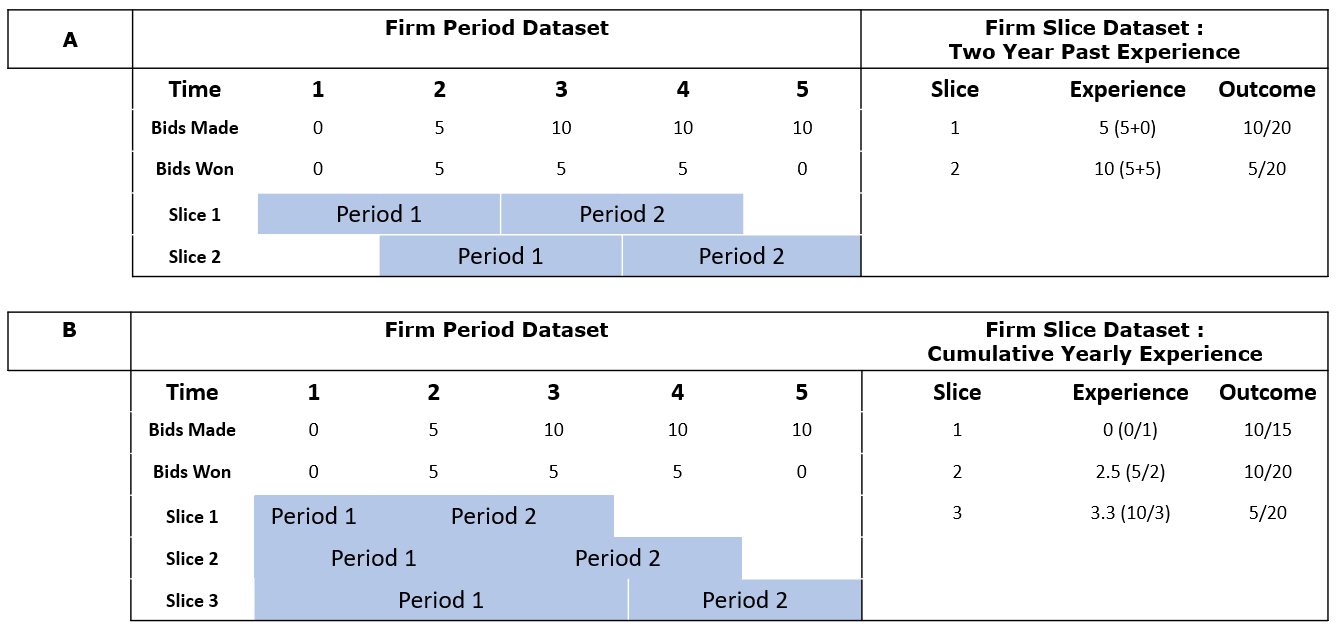
\includegraphics[scale=0.53]{diagram_experiences.png}
  \caption{Example computation of slice-firm dataset, employing two-year fixed periods of past experience (A), and cumulative yearly experience (B).}
  \label{fig:diagram_experience}
  \vskip 0.5mm
  { \footnotesize \underline{Note:} }
\end{figure}

Finally, we add period fixed effects for each period of outcomes being considered to control for changes in the market environment throughout the sample.

%In some specifications we include firm fixed effects based on size. It is possible that smaller firms face higher competition due to less-complex contracts, and so their baseline level of success in the market will be lower.

After the transformation steps, we obtain five slice-firm datasets for the first measure of experience and six slices for the second measure of experience. The following table shows the amount of observations in each slice by the type of experience measure employed. Recall that every observation is a firm-level aggregate of past experience and summary of future outcomes and have the form of the righmost table in Figure \ref{fig:diagram_experience}.


%The OLS regression in equation may have endogeneity problems. This next section discusses the sources of the problem and the identification strategy.


\subsection{Endogeneity and Identification}
Causal interpretation of the regression in Equation \ref{eqn:olsspec} is problematic since unobserved cost variables, specific to each firm, are omitted in the regression (since they are unobservable) and also endogenous. If there are highly efficient firms which due to this advantages are able to bid more aggressively or submit better proposals, they should win more projects, and in turn accumulate more experience. We expect our estimate $\hat{\beta}$ (coefficient on experience) in \ref{eqn:olsspec} to be biased upwards due to correlation (expectedly positive) between omitted cost variables and the amount of past experience.

To identify the causal effect of experience on outcomes, one alternative is to employ external variation to instrument the experience of a firm in an Instrumental Variables (IV) approach. We discuss what would be the optimal way of producing external variation, and, since the data does not allow us to employ this strategy, we propose two second-best alternatives.

Ideally, one could use close wins as the source of exogenous variation in past experience. The argument is that close wins should be less or not at all attributed to unobserved cost factors, or other efficiency advantages, but instead attributable to random differences, for example, the conservativeness of each firms' engineers' estimates. The optimal way to identify close wins would be to single out auctions for which the winning firm had a final weighted score which was marginally superior to the next (or several) of its competitors.  Recall that, for each contract, the  proposals from firms are scored in several criteria, weighted, and finally summed to produce the total score for that firm.

In this approach, our first stage takes the form of Equation \ref{eqn:firststage} . Here $EXP_{it}$ is the total set of contracts won in slice $t-1$ for firm $i$, while $EXPCLOSE_{it}$ is the subset of the contracts won which was won closely as per the definition above, and $\nu_{it}$ is an error term uncorrelated with $EXPCLOSE_{it}$.

\begin{equation}
\label{eqn:firststage}
EXP_{it}= EXPCLOSE_{it}+T_t+\nu_{it}
\end{equation}

The second stage is shown in Equation \ref{eqn:secondstage}.

\begin{equation}
\label{eqn:secondstage}
EXP_{it}= EXPCLOSE_{it}+T_t+\varepsilon_{it}
\end{equation}

Clearly, both measures of experience ($EXP$ and $EXPCLOSE$) are correlated since every extra unit of experience increases the probability of having at least one close win. Moreover, close wins should not be correlated with cost measures, as they are attributed to random factors, such as risk-aversion differences between firms, random approximation differences between engineering teams in each firm, etc. and thus we should also have a valid instrument.

Unfortunately, the previous strategy is unfeasible a with the data we have avalaible. Our data only allows us to see the criteria employed in each contract and the weight of each factor, but not the individual scores for each firm. We attempt two alternative methods detailed in the subsections below

\subsection{Close wins by close bids}
 The first method follows the same theoretical setting as before, but changes how close wins are singled out. Close wins are now operationally identified as the wins meeting copulatively  three conditions: i) the price weight in the awarding decision criteria is 70\% or higher ii) the contract was awarded to the lowest bid and iii) the difference between the lowest bid and the second lowest bid is less than .05\%. We expect that this way of identifying close wins does indeed capture a subset of the random wins, namely, random wins in projects where price is the major awarding criteria.

This definition of close wins leads to approximately 8\% of winning bids being classified as a close one. In the robustness checks, we also consider a different values for these parameters, where we consider close wins where three or more competitors are all within a 1\% difference in their bids.

In the next table we examine whether close wins defined as  above are different from the population in several types of metrics. We can see that in most aspects these bids are not exceedingly different from the rest of the sample, so we expect that there are no underlying project characteristics that could affect competition for these contracts.

\begin{table}[!h]
\caption{Comparison of key statistics between close wins(<0.05\% difference between 1st and runner-up) and regular wins}
\centering
\resizebox{\textwidth}{!}{
\begin{tabular}[t]{ccccc}
\toprule
Variable & Mean (Not close win) & Mean (Close win) & Sd (Not close win) & Sd (Close win)\\
\midrule
Bid & 6.3e+08 & 3.32e+10 & 1.06e+10 & 8.11e+12\\
Bid\_Winning & 3.18e+08 & 2.37e+08 & 3.56e+09 & 2.62e+09\\
Difference between 1st bid and 2nd (\%) & 0.14 & 0.0186 & 0.115 & 0.0147\\
Number of Bidders & 3.86 & 4.08 & 2.12 & 2.23\\
Year & 2020 & 2020 & 2.92 & 2.89\\
Offers made by Firm & 4.4 & 6.17 & 7.34 & 11.2\\
Win prob. by Firm & 0.191 & 0.171 & 0.3 & 0.274\\
Offers won by Firm & 0.972 & 1.37 & 2.1 & 3.23\\
\bottomrule
\end{tabular}
}
\end{table}

\subsection{Close wins as close rank}
There coul two main objections to the previous identification strategy:
\begin{itemize}
  \item The price is not the only awarding factor. Thus, it is possible that even in a contract where price is a major component, the cost advantages of a firm manifest in terms of other awarding factor, like quality. That is, the firm offers similarly priced goods but at a much superior quality.
  \item The closeness between the first and the second bid does not take into account the full pool of participants.
\end{itemize}

We propose a new alternative to identify close wins which does not rely in prices or any other aspect of the bid itself. Instead, we label for any winning given firm a close win if all the firms involved in the auction were close in ranking. The argument here is that, given a well constructed ranking, winning a contract against closely placed opponents is attributable to random factors.

Obviously, the main issue is how to construct a good ranking measure. We proceed by  modeling each auction as a multi-player game event (in the non-economic sense of the term) in which firms gain points by winning the project and lose points by not winning it. We award and substract points based on a modified ELO algorithm suited for multi-player games.

Each firm has its ranking initialized at a pre-specified level (1,500 in the initial version). Then, it is awarded 24 points for winning againsta a similar oponnent and substracted 8 by losing. The implementation of the algorithm recommends that points awarded and substracted sum to zero, so we fix awarded points and choose substracted points such that on average (given the number of players in an auction) this condition holds. Against non-similar opponents, the algorithm makes a correction based on the ranking of the players and the outcome of the game. The details of the algorithm are given in the Appendix.

Proceeding from the oldest to the most recent auction, we update the initial rankings for each firm and obtain for each firm its ranking at any point in time. Next, we label a win as a "close win" when the highest rank among the bidders for the auction was not more than 3\% higher than the lowest rank among the same set of bidders. This yields around 7,322 closely won contracts (16\% of the contracts in the analysis sample) which corresponds to 21,763 observations (16\% of the observations in the analysis sample). In Table \ref{tab:closewins_alt2_desc} we present summary statistics for close wins identified via close wins.

\input{C:/repos/learn-doing/thesis/tables/table_closewins_alt2_desc.txt}

In the analysis, for our first measure of experience we drop the first slice of data outcomes (as defined above) to allow for a period of rank adjustment. This is necessary since the algorithm does not work well when the average rank in the population is not clearly defined. The way ranks evolve as we progress in the time of the data can be seen in Figure \label{fig:rankings_times}. Note that ranks appear concentrated at the end of the first year of data, while much more dispersed at the end.

\begin{figure}
  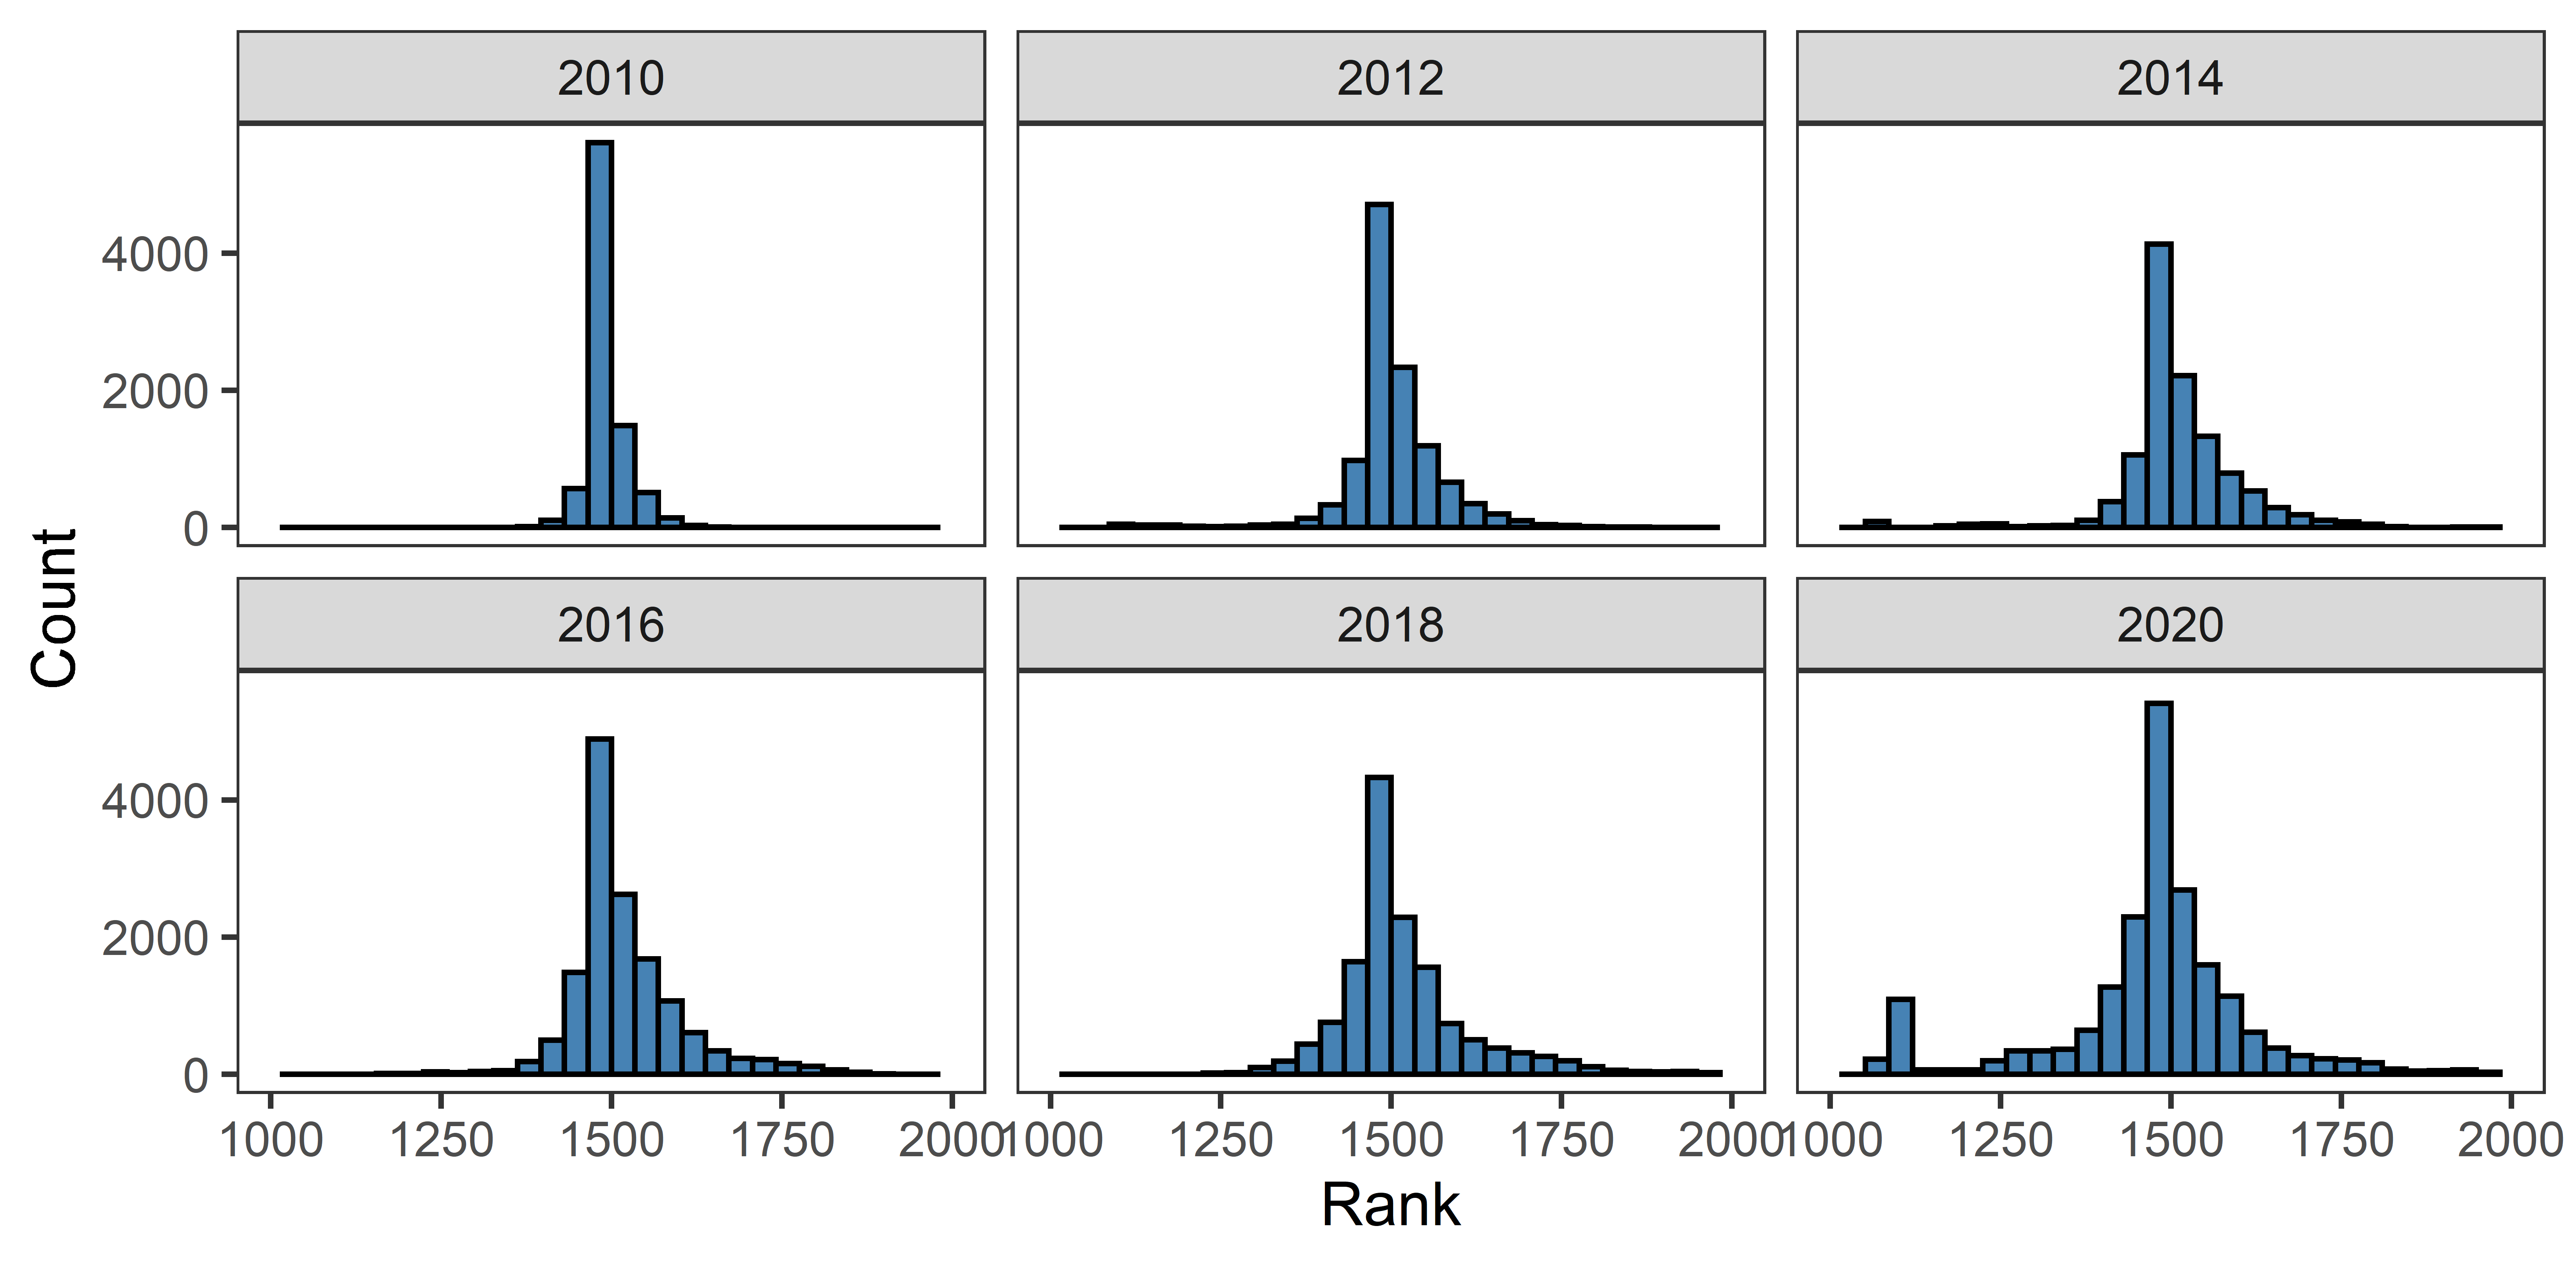
\includegraphics[scale=0.95]{rankings_times}
  \caption{Evolution of ranks by selected years}
  \label{fig:rankings_times}
  \vskip 0.5mm
  { \footnotesize \underline{Note:} \par}
\end{figure}

In the robustness checks we analyze both i) different values for the won/lost points after an auction and ii) the threshold in ranking for a close win.
%Bidding behavior
%An alternative way to measure changes in bidding behavior caused by efficiency gains through experience is to examine directly changes in bidding behavior among more experienced firms with respect to less experienced ones. As was discussed before, experience induces changes in the underlying production function, or changes along the production function, that make the firm more efficient at producing certain types of goods. In a competitive market, firms should pass through at least a fraction of this improvement in costs to the bids they submit in the auctions. Thus, we should be able to identify this change directly through the bids that more experienced firms submit for projects.
%The approach is different than the one from the previous section because we can directly link the past experience of a firm to each bid it submits in every auction that it participates in. Thus, our unit of observation is a bid submitted by a firm for a contract of a public construction contract. Our second specification has then the following form:where is the standardized bid submitted by the firm and is a measure of past experience. In further specifications we include a broader set of controls. First, we add fixed effects by auction. Second, we add firm fixed effects. Finally, we control by the geographic region where the auction is being held.
%The outcome variable is the standardized bid submitted by firm to the auction, i.e. the original bid amount divided by the engineering estimate of the project. This approach allows us to make comparisons along project of different sizes. It is also useful because it should be expected that our dependent variables have effects per unit of contract amount (Bajari, 2010). The standardization also controls for some sources of heterogeneity.
%The dependent variable is the total number of contracts that the firm has won up until the moment that the firm submits its bid. Since for the first periods in the data we do not have information on past experience, we exclude the first two years from our observations of outcomes and only employ them to compute experiences for firms from year three and onward. In the robustness section, we explore several alternative ways to measure experience and subset the set of firms.
%In the same way as before, we expect that there will an endogeneity between cost measures and bidding behavior. We should expect that firms which have a baseline efficiency higher than other firms will be able to submit lower bids and gain more experience, so we could pick up effects of reverse causation in our coefficient for experience.  We thus employ a similar Instrumental Variables approach as before, instrumenting total past contract wins with close contract wins.

\section{Main Results}

First we explore graphically the relationship between our first measure of experience and outcomes. Figure \ref{fig:plotresults_both} , Panel A, shows the relationship between past experience and outcomes (i.e. winning share). While we can see an increase in the average share of contracts won with more past experience, there is considerable heteregeneity, as it can be seen in the wide error bars (which show interquartile range). Panel B contains only two types of firms: firms that either bid but not won contracts in period $(t-1)$ or firms which won one or more close contracts in period $t$, and thus is akin to results of a reduced form regression.

\begin{figure}
  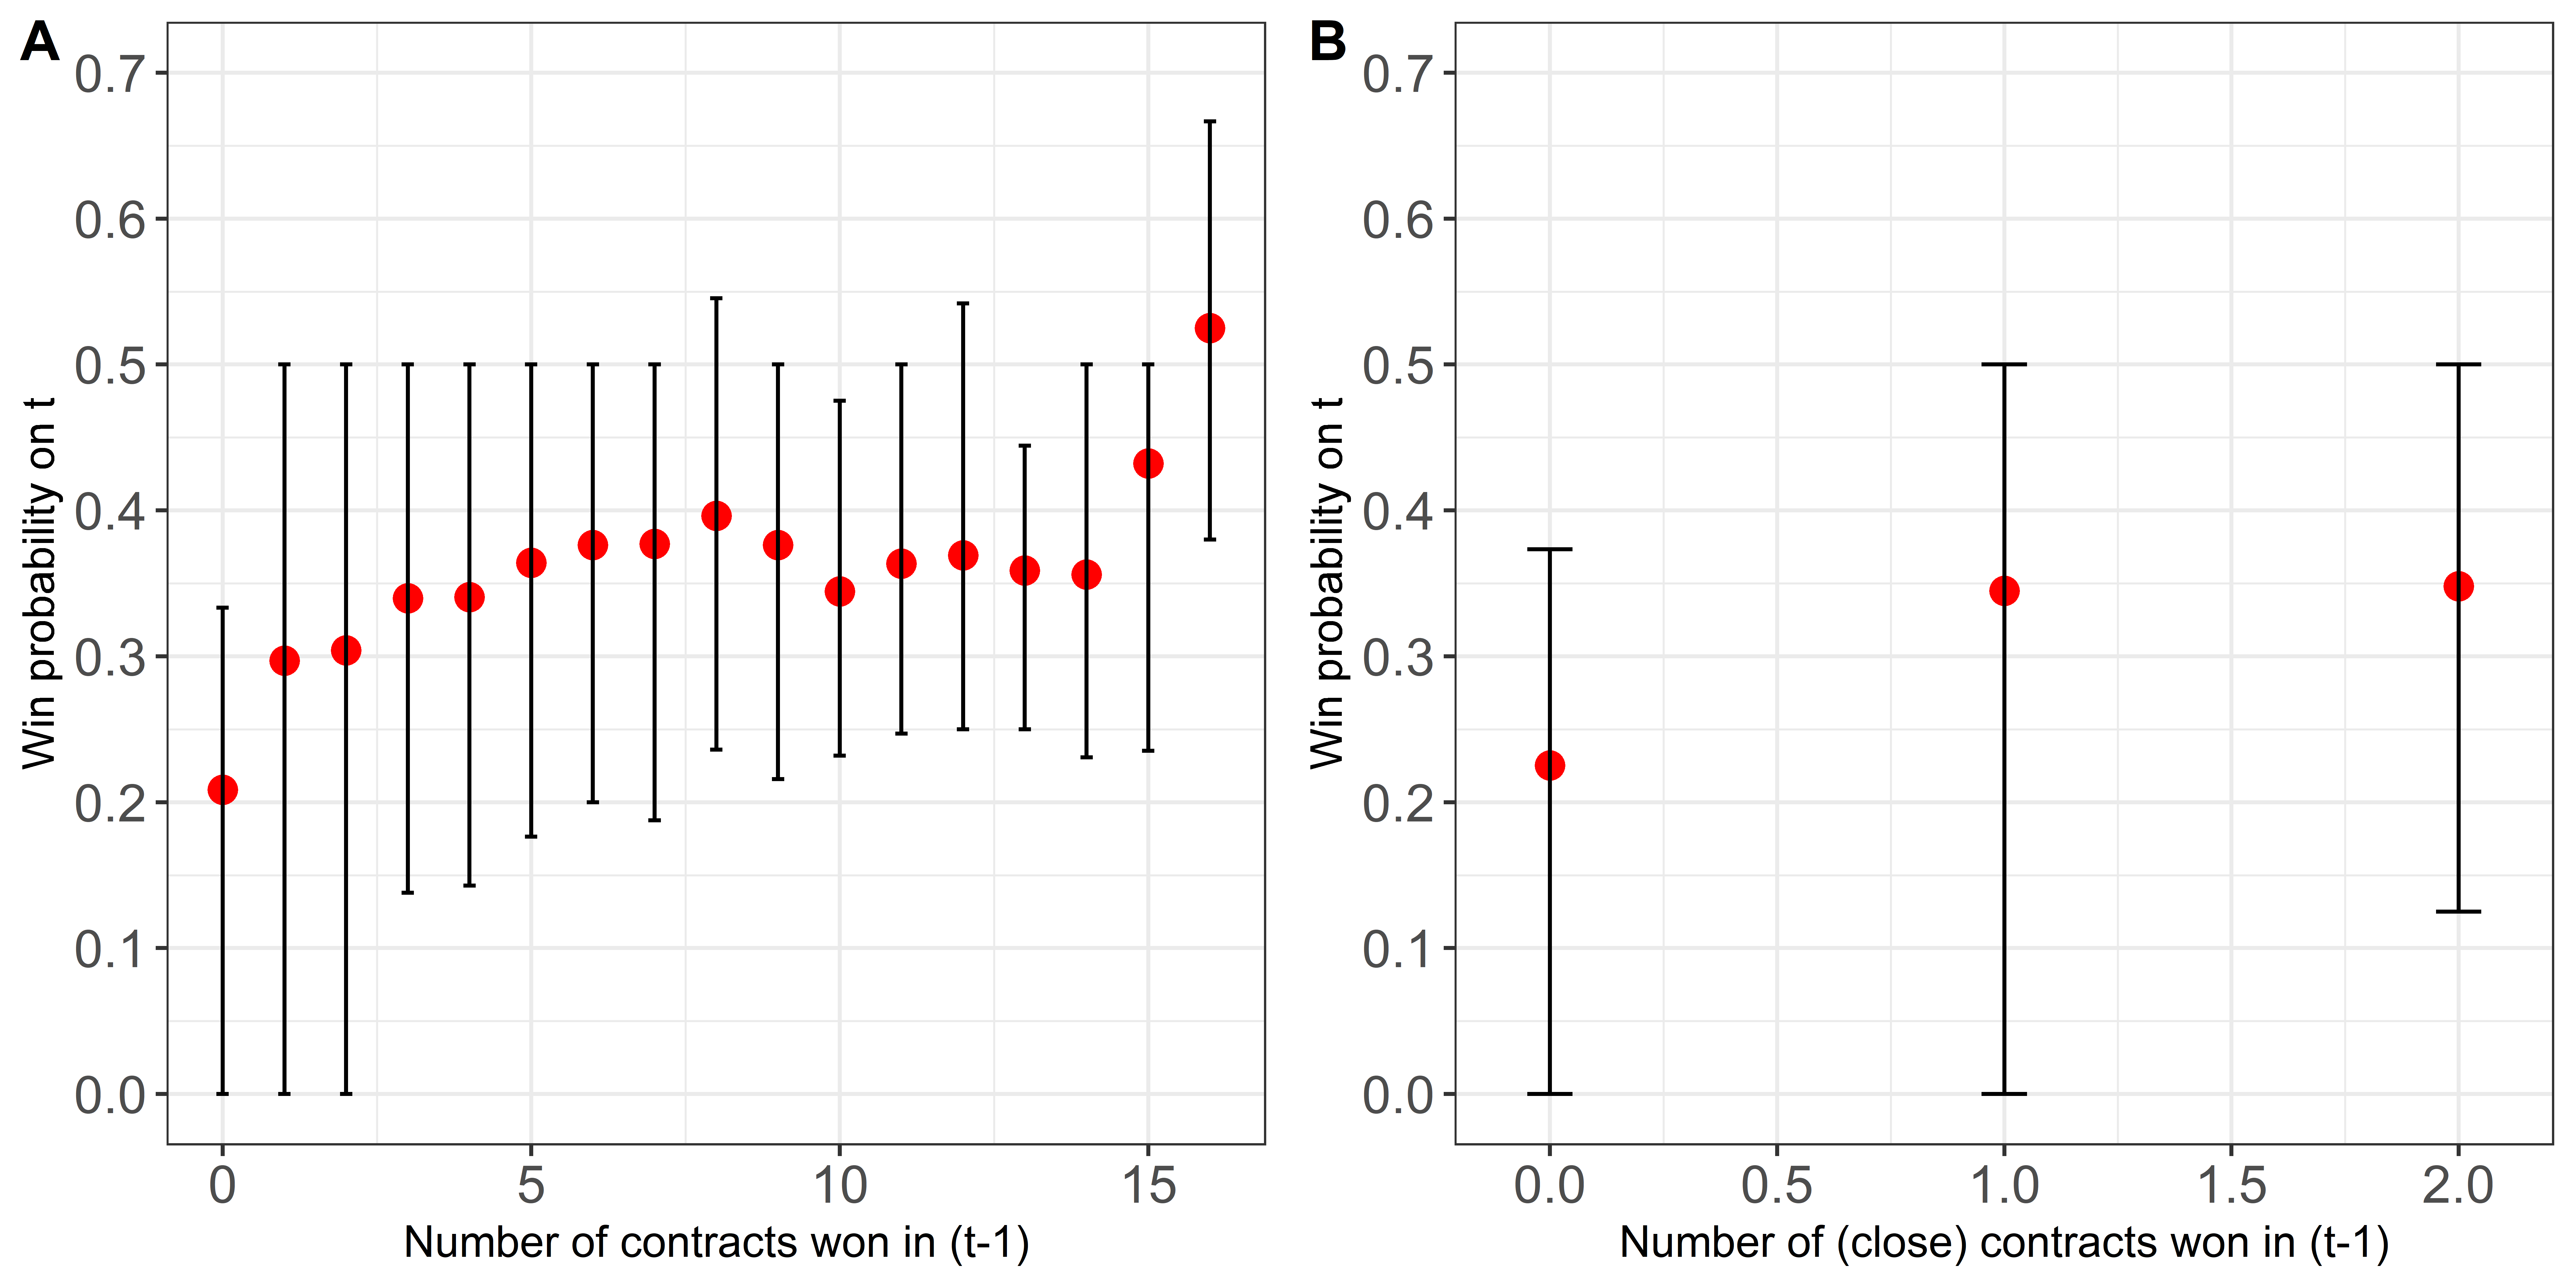
\includegraphics[scale=0.65]{plotwins_both.png}
  \caption{Relationship between contracts won on $t-1$ and mean winning probability across contractors in $t$.}
  \label{fig:plotresults_both}
  \vskip 0.5mm
  { \footnotesize \underline{Note:} The plots show the mean across firms of the number of contracts won out of the number of contracts bid for in period $t$ (in the $y$-axis), against experience accrued in period $(t-1)$ in the $x$-axis. $t$ and $t-1$ correspond to two periods of two years each. Since the data contains ten years, the observations correspond to outcomes computed for eight outcome periods.  Only $x$ for which the number of observations is greater than ten are shown. Error bars correspond to the interquartile range. Panel A: all sample observations are considered. Panel B:  shows results for a subsample where the only contractors considered are those who either i) won closely one or more close contracts  on period 1 or ii) did bid but not win a contract in period 1\par}
\end{figure}

Table \ref{tab:table_exp_1} shows the results for OLS and IV regressions for our first experience measure (i.e. rolling two year periods) while Table \ref{tab:tableExp2} shows the results for our second measure of experience (i.e. annualized experience).

In both tables, OLS results are in the first to third panels. The first panel shows that the OLS coefficient on the effect of having any level experience against not having experience (binary) is around 0.10, for both ways of computing experience (and ). Our specification with linear returns on experience shows that experience renders a 0.02 and 0.05 increase in winning share per extra contract developed (for experience measures 1 and 2 respectively). All the estimates for the experience-related coefficients are significant at $p=0.01$ with robust standard errors.

The IV results (fourth to sixth panels in each table) show that  the linear and quadratic estimates of the coefficients on experience generally stay within $\pm$ 0.03 of their OLS counterparts. There is however an increase in the binary measure of experience coefficient, for both measures of experience, since for the first measure of experience \textbf{this rises from and for the second measure this rises from} . This is different than we expected, as our initial concern was that omitted cost variables would bias estimates upwards.

A concerning result is the low $R^2$, which shows that altough the effect of experience on the mean outcome is significant, there is much variability among firms' outcomes which is not explained by experience.

\input{C:/repos/learn-doing/thesis/tables/table_ols_exp1.txt}

\input{C:/repos/learn-doing/thesis/tables/table_ols_exp2.txt}

There does not seems to be conclusive evidence regarding different results when employing quadratic rather than linear functional forms for experience. For example, Figure \ref{fig:pred_average} shows the mean confidence intervals, employing as period fixed effects the last period in the sample. It can be seen that the fitted total predicted value does not seen to vary greatly from the linear to the quadratic specification.

\begin{figure}[H]
        \centering
        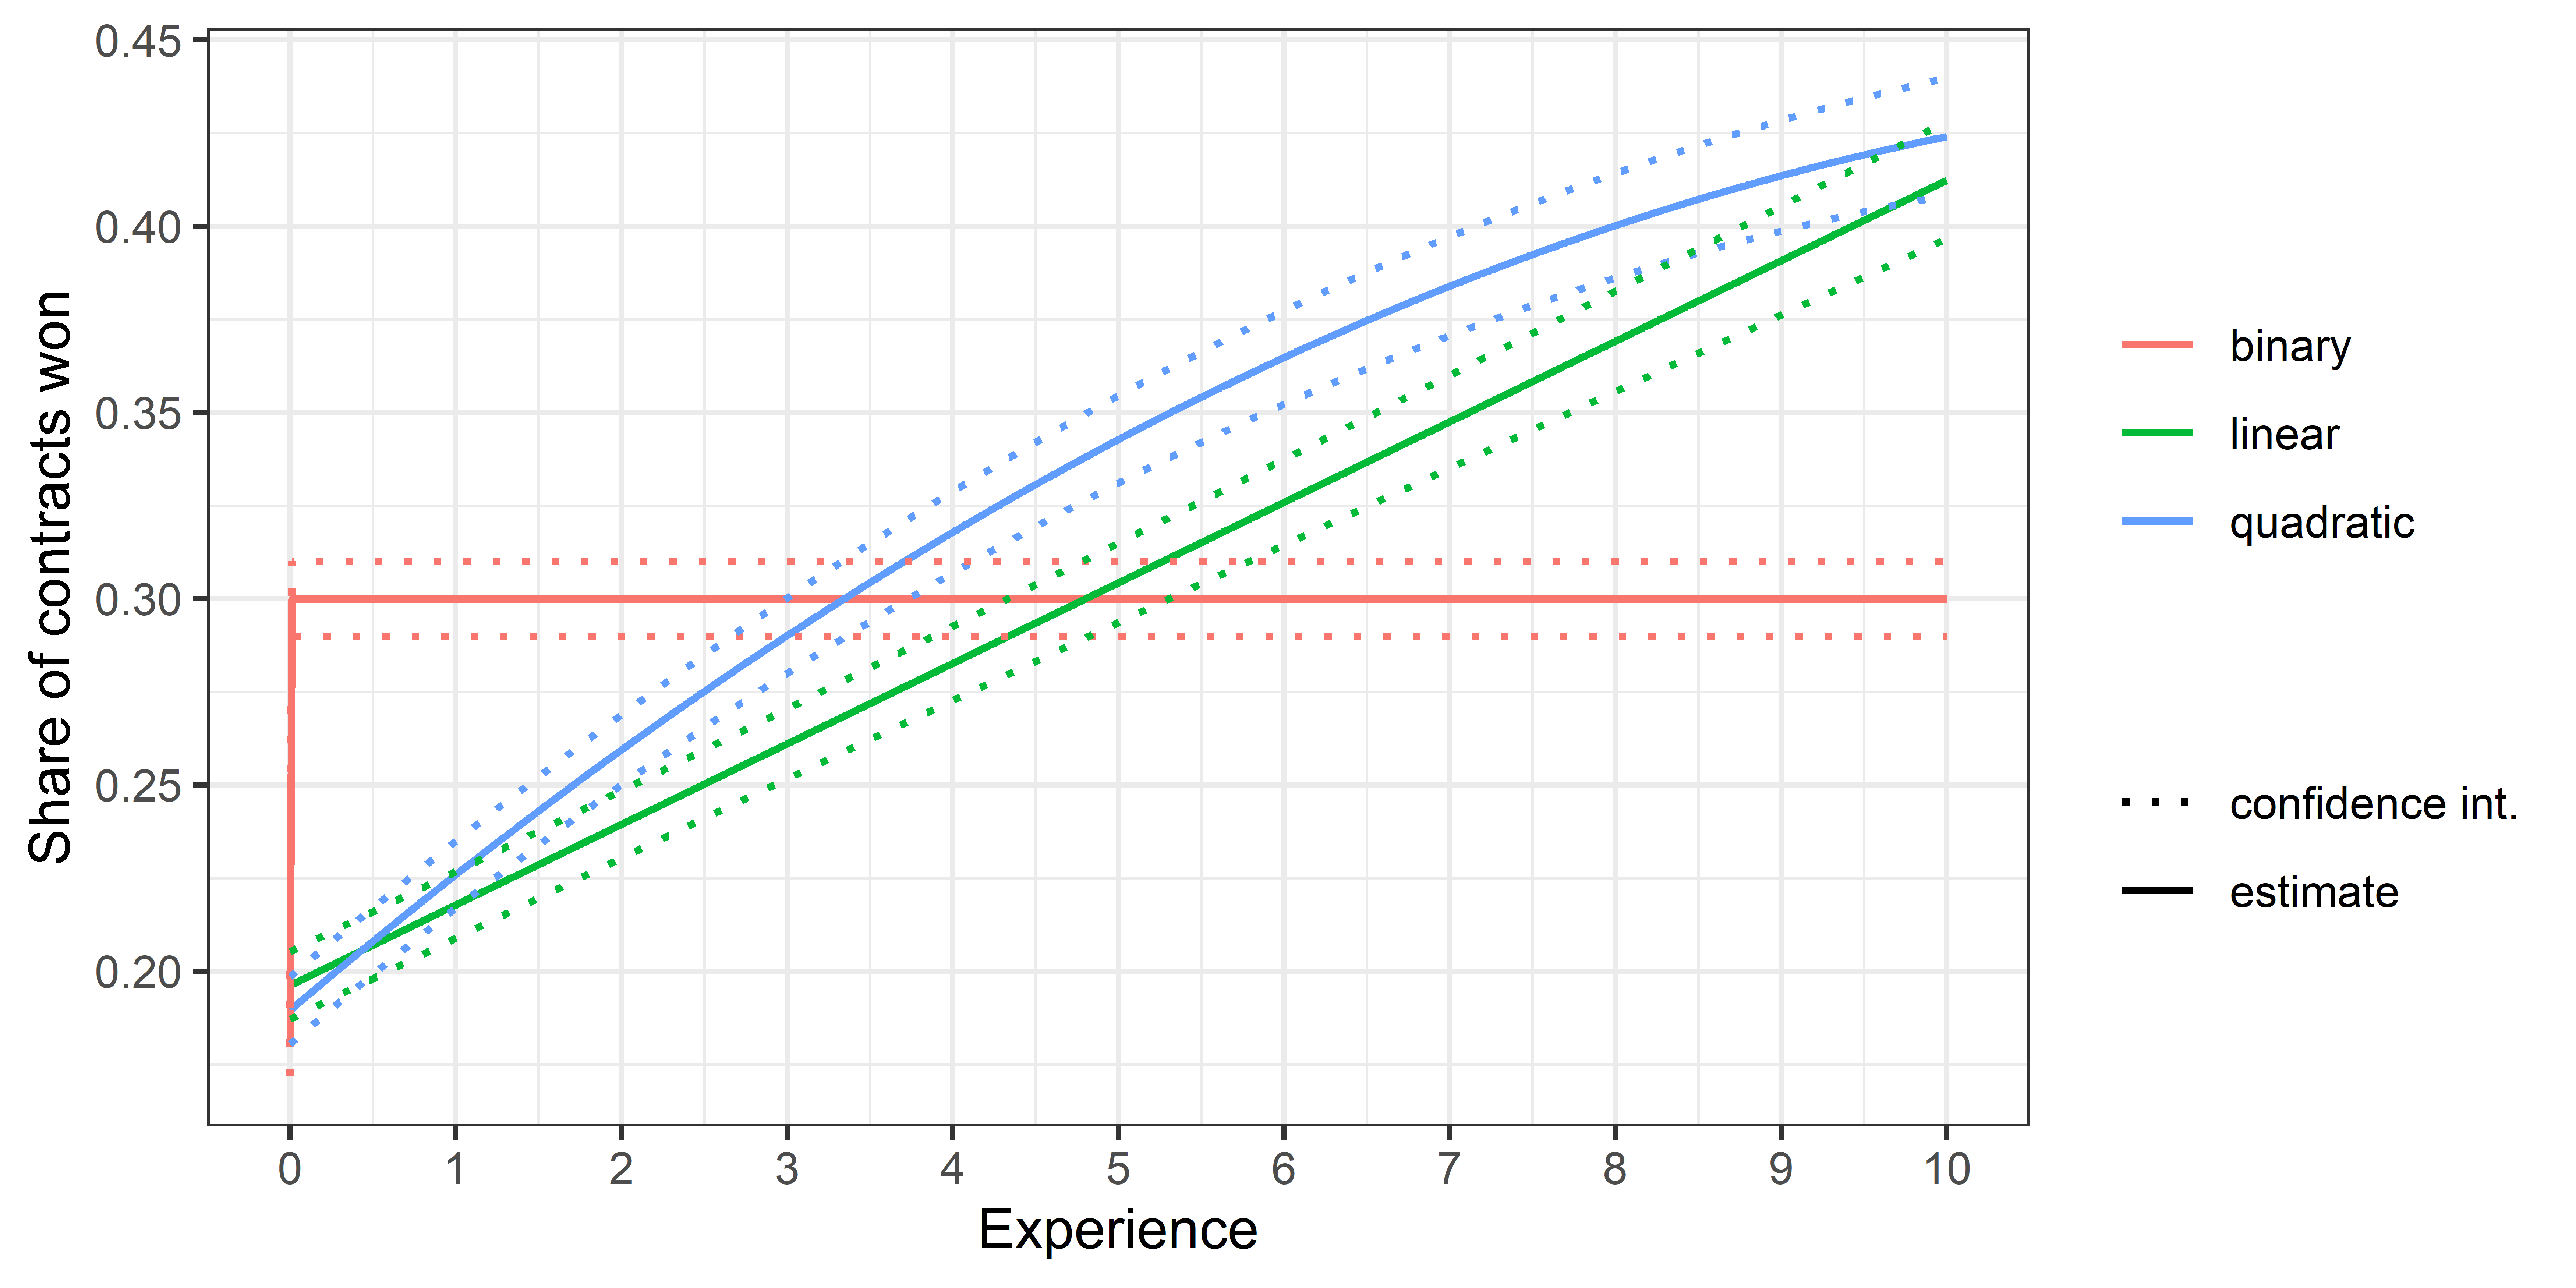
\includegraphics[scale=0.8]{fit_sample.png}
        \caption{ \small Predicted values for the mean of the outcome variable (share of contracts won), by total experience accrued in the previous period. We employ fixed effects as in the last period of the dataset.}
        \label{fig:pred_average}
    \end{figure}




\section{Experience and Type of Project}
Given our previous results a natural concern is if whether all projects exhibits the same returns to experience or if experience is more important in certain types of works. In this section we replicate the previous analysis by disaggregating by type of project. In order to do this, we classify certain projects according to their description, then run similar regressions as in the last section, and present the results.

First we describe briefly how we construct categories for the prrojects and which ones are avalaible for the analysis. Our original dataset includes a name variable which describes the type of project with some extent. We extracted this name variable and looked for i) common single words (unigrams) and ii) common pairs of words (bigrams). We select the most common unigrams and bigrams and map similar words and bigrams to project categories. The full categorization mapping can be found in the Appendix.

We end up with contract classified under categories. Importantly, if a contract includes unigrams or bigrams in its name belonging to more than one category, it is included in the analysis of both categories. The number of contracts, average amount, average number of bidders for each category is shown in Table \ref{}. We can see that the biggest categories of projects are school-related, vecinal works, parks and pavements (including sidewalks). The Appendix contains more details on the types of projects included in each category.

%\input{C:/repos/learn-doing/thesis/tables/table_types_project_stats.txt}

Next we run similar regressions as in the previous section for each project type, considering as our dataset only the contracts in that project category . We employ the same specification of with a linear functional form on experience and period fixed effects, and our first measure of experience. The results are presente in Figure \ref{fig:typeestimates}he Appendix includes more detailed tables with full regression results for each sproject type. A few results stand out. First, we get the biggest coefficients on experience on graveyard projects, footbridges and housing. The first two should be almost exclusively procured by government units. Housing was also one of our hypothsized types of projects which should have high coefficients. At the bottom of the distribution, interestingly, we find daycares, sports courts, hospitals, and schools. The results could be explained because these projects are mostly composed of normal construction works which also have private close substitutes.

The results on hospitals should be surprising, as they are usually very big projects with a lot of specific knwoledge required.

%\input{C:/repos/learn-doing/thesis/tables/table_types_project_ols.txt}

\begin{figure}
  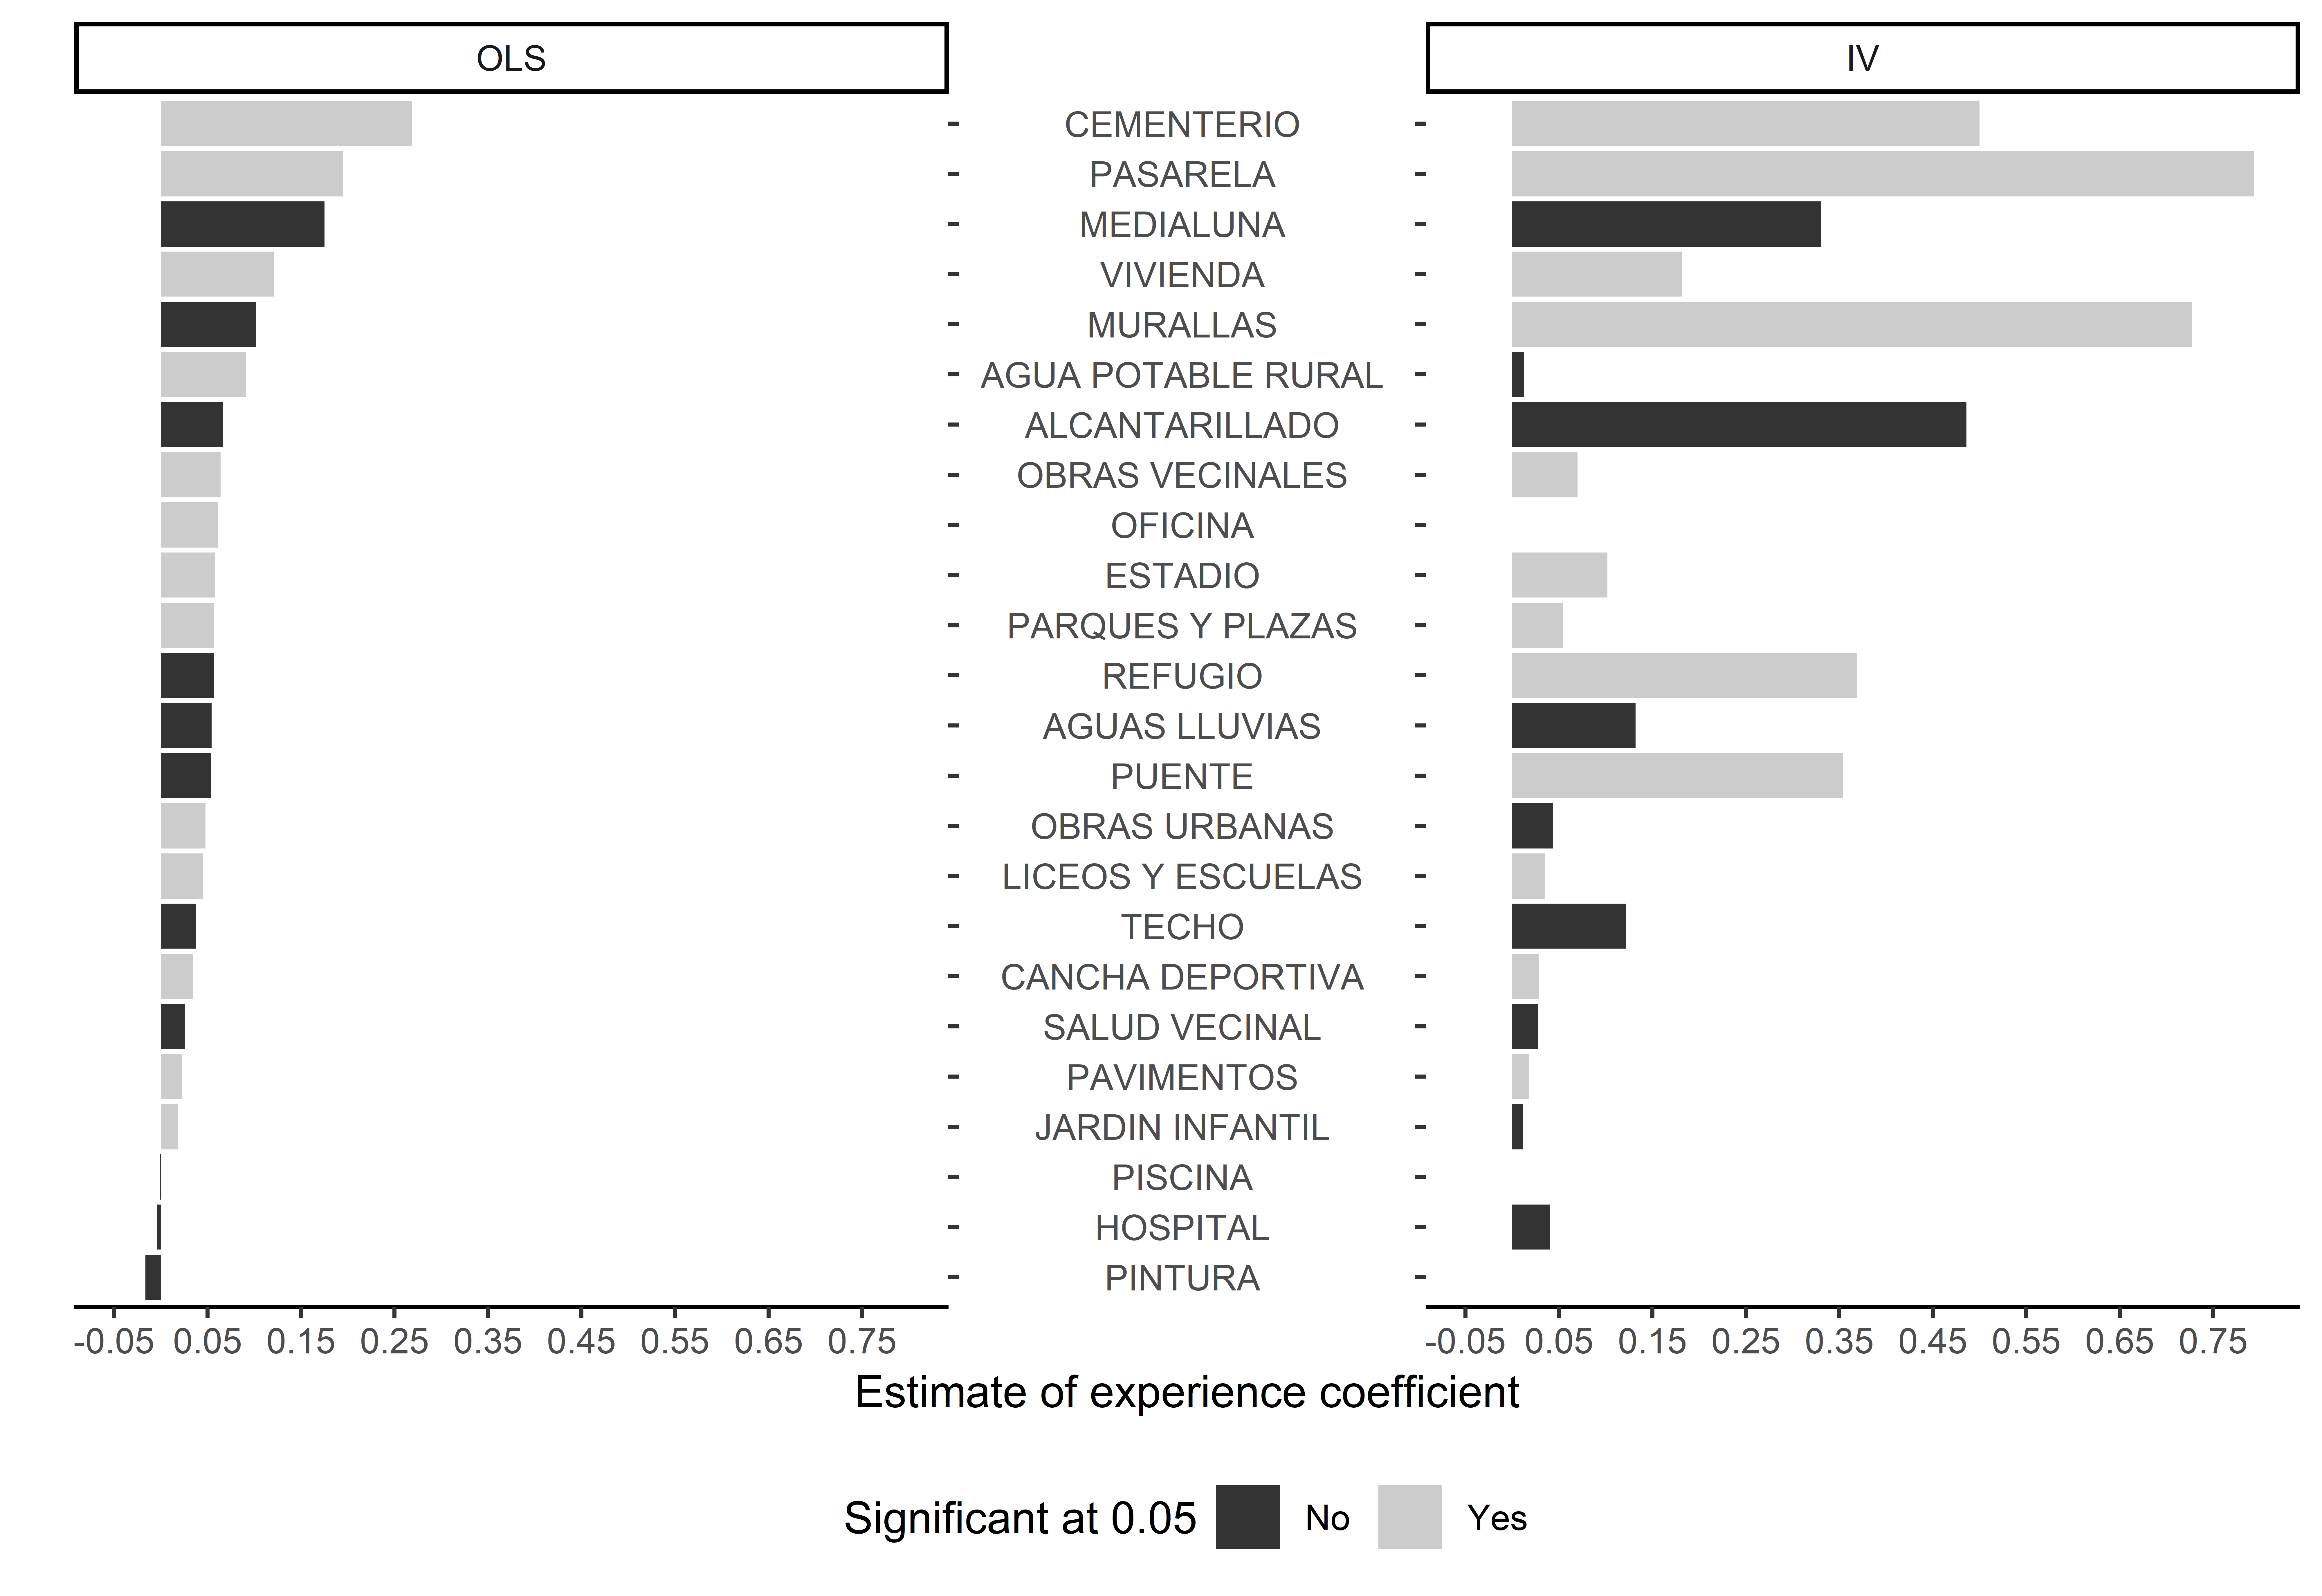
\includegraphics[scale=0.75]{plotTypes.png}
  \caption{Experience coefficient by type of project.}
  \label{fig:typeestimates}
\end{figure}

\section{Experience and Firm Size}
%In the literature about industrial organization and productivity, it has been studied the relation between firm size, innovation, and productivity. These investigations have concluded that smaller firms are more productive than bigger firms, however they are also more risky.
An important variable in the investigation of the effect of experience should be firm size. First, it is possible that there are different levels of cost efficiency between small and big firms. As arguably bigger firms should have more experience on average, this could skew our estimates. A second concern is that we might expect experience to matter more for smaller firms, if there is a decreasing or "maximum" level effect of experience on future outcomes.

In this section we attempt to develop specific estimates of the effect of experience for different levels of firm size. Developing intra-category estimates serves as both as an identification strategy and as  robustness check of our previous findings.

 We follow the following approach. First we select a subsample from our original dataset which we can classify acoording to annual sales.  We obtain intra-category estimates of the effect of experience and interpret them. Finally, we discuss the results and some of the empirical challenges of controlling for size.

In order to study and control for firm size we employ a publicily avalaible classification of firms according to their annual sales, maintained by the chilenan Tax Bureau Office (\textit{Servicio de Impuestos Internos}). Firms are categorized in 13 categories. Category number one  corresponds to 'tax data not enough to classify', but from categories two up to thirteen, each category is defined by an increasing level of minimum yearly sales.

This data is avalaible only for firms not being fully assimilable to final taxpayers. After merging our with our initial sample, we are left with around 30\% of our original firm sample. Table \ref{tab:salescategories} shows how many firms do we have in our sample for each category, average annual sales for these firms, and statutory annual sales thresholds for each category. Note that we have much more firms at intermediate categories than extreme ones. In our estimation we group firms from contiguous groups together to increase power.

% Table generated by script
\input{C:/repos/learn-doing/thesis/tables/table_tax_categories_data.txt}

We estimate the effect of linear experience with our first measure for each group of categories of firms by OLS and IV. Specifications consider our first measure of experience with a binary presence of experience and with period fixed effects. The results are presented graphically in \ref{fig:sizeestimates} (the coefficient for category two is omitted because it was much bigger than the rest and distorted the visualiztion). Full results are avalaible at the Appendix.

We only obtain significant effects at intermediate sales categories' levels. However, everytime a coefficient is significant it is also positive. The results are not supreising given i) the reduced sample we are employing ii) the expected reduced importance of experience for very big firms.

Controlling for firm size is challenging mainly because of statistical reasons. First, firm size distribution in the sample is not uniform as there are less very small and very big firms. Second, the within-size distribution of experience within extreme categories has very few observations with more than five contracts of experience. Third, this sample is already smaller due to filtering single-person companies. Both factors make it hard to obtain per-category estimates with enough statistical power experience.

\newpage
\input{C:/repos/learn-doing/thesis/tables/table_firm_sizes_intercepts.txt}


%\begin{figure}
%  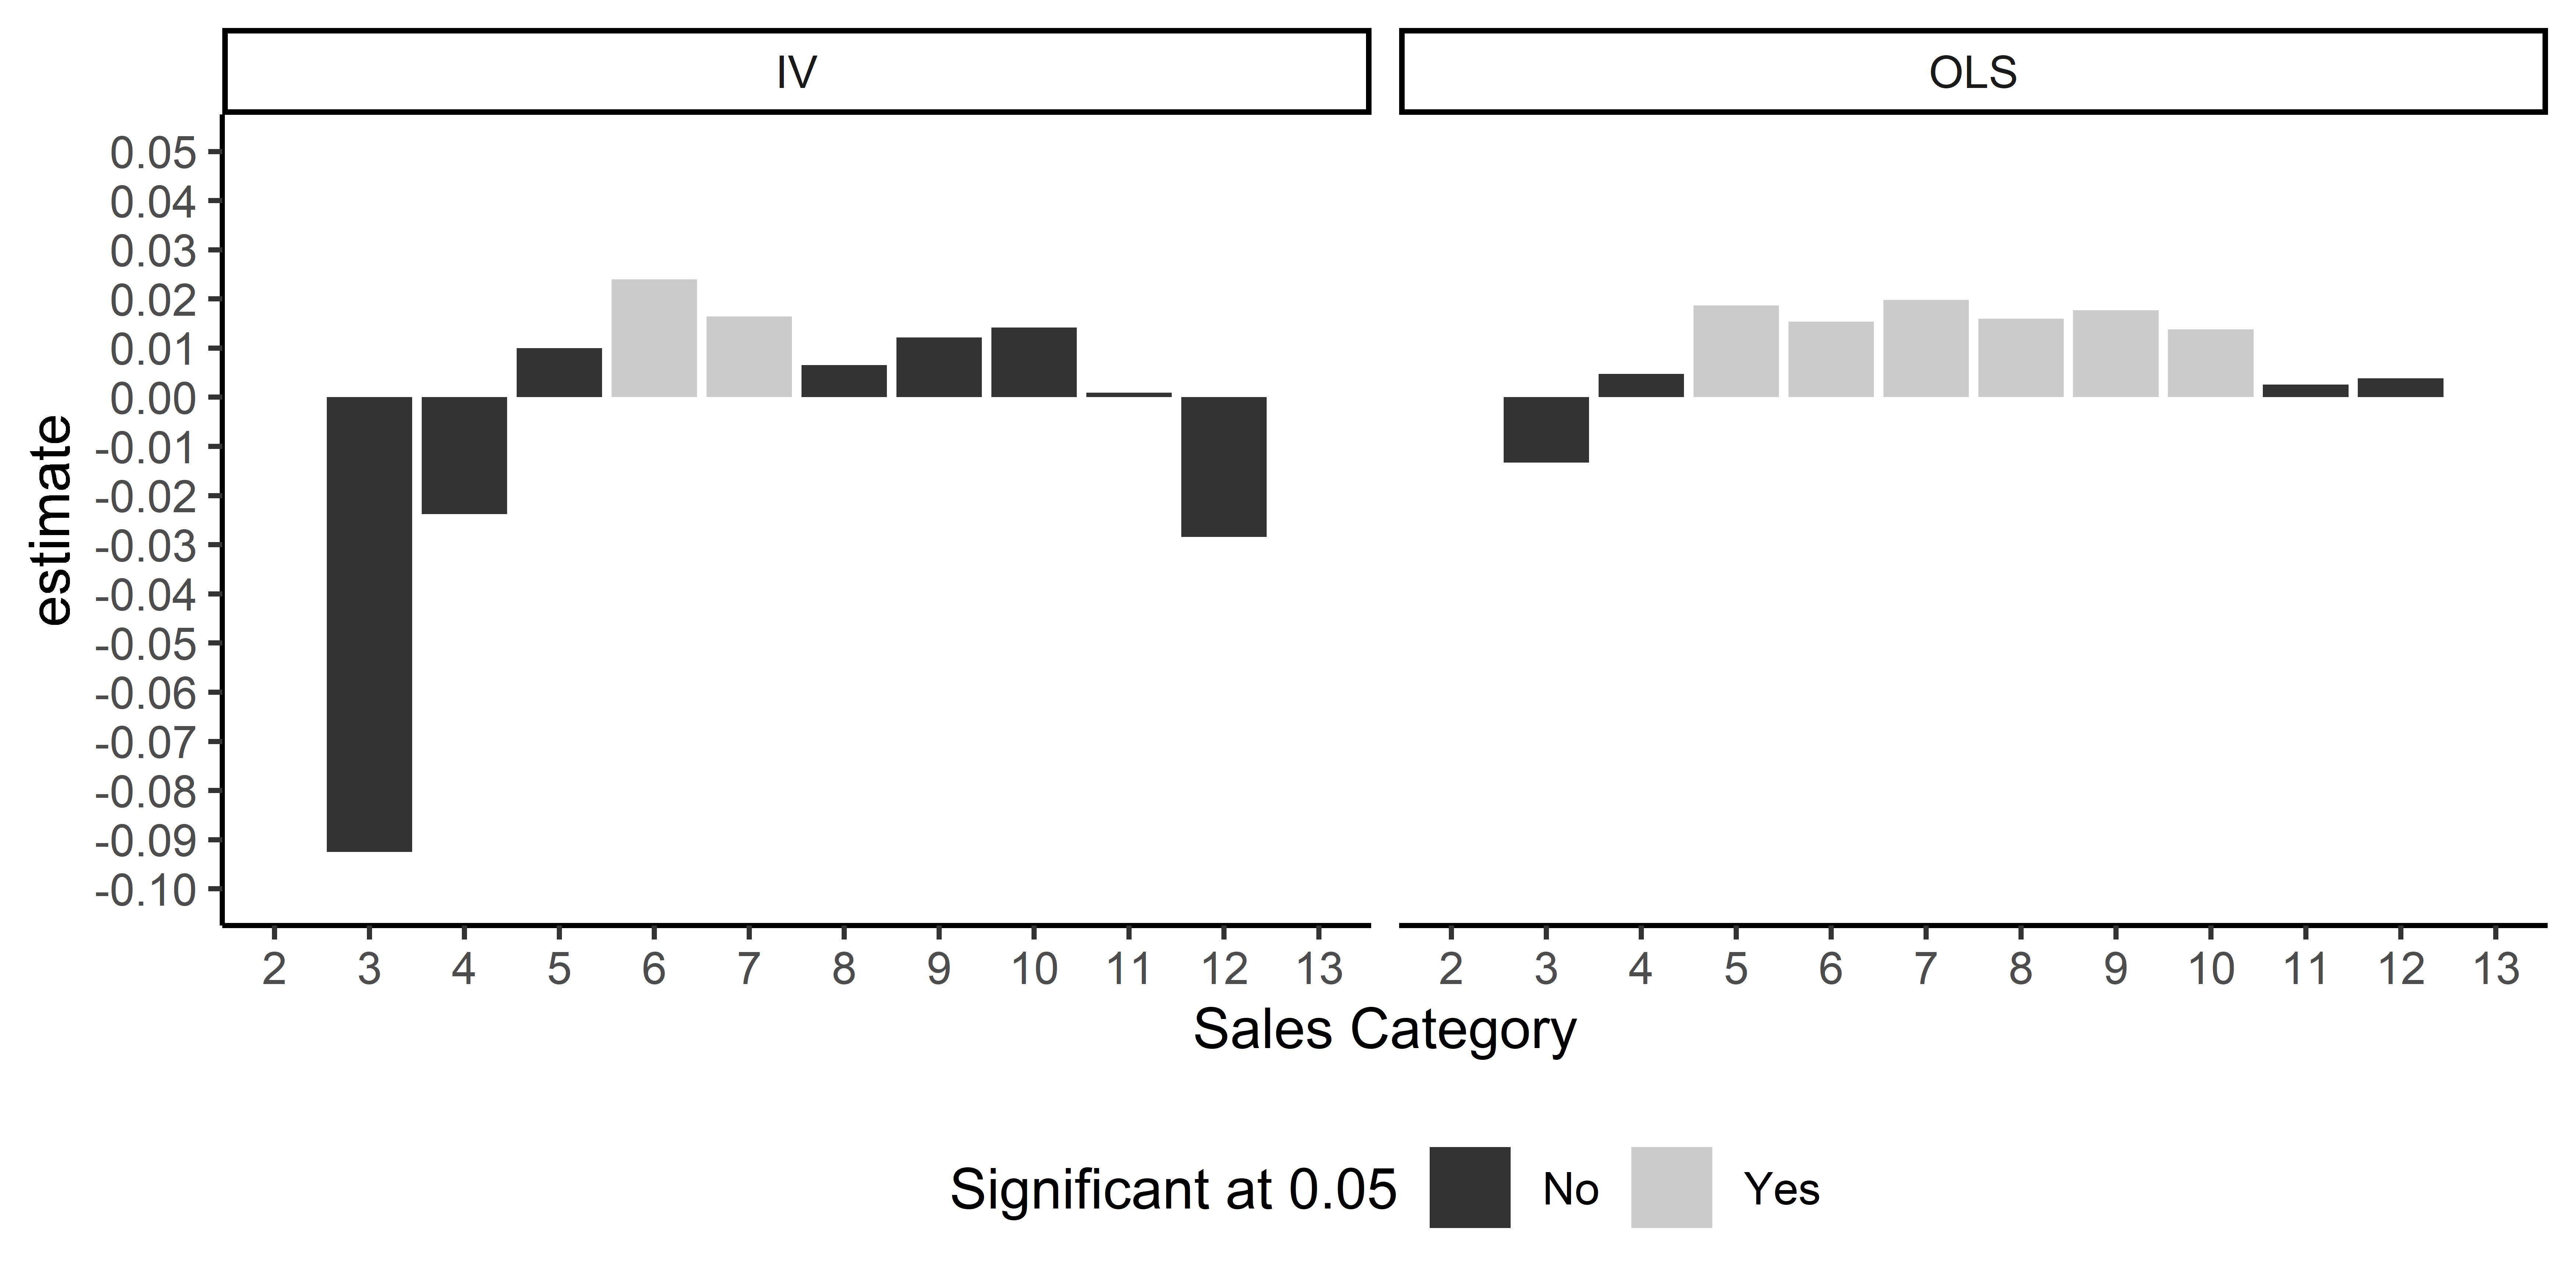
\includegraphics[scale=0.85]{plotsize.png}
%  \caption{Experience coefficient by tax sales category}
%  \label{fig:sizeestimates}
%\end{figure}


%\resizebox{\textwidth}{!}{%
%\input{C:/repos/learn-doing/thesis/tables/table_sizes_explinear1.txt}
%}%
\section{Robustness checks}
Several of our choices in the previous section admit several arbitrary choices. In this section we consider several extensions in parameters which could influence the results obtained before. We consider robustness checks in the following areas:

\subsection{Periods of outcomes}
In the previous section, we measured outcomes occuring in two year periods. We now consider outcomes occuring in one and three year periods as well. Note that in this part we only vary the length of the period where outcomes are computed and we maintain the procedure to compute experience as before. Table shows outcomes computed for periods of 1, 2(the original specifications) and 3 years. The first three columns employ the experience measured in the two-period previous to the outcome period while the 3-6 compute experience as annualized cumulative experience as discussed in the previous section.

\begin{table}[!htbp] \centering
\caption{Regression for OLS and IV specifications}
\label{}
\resizebox{\textwidth}{!}{%
\begin{tabular}{@{\extracolsep{5pt}}lcccccc}
\\[-1.8ex]\hline
\hline \\[-1.8ex]
& \multicolumn{6}{c}{Contracts Won/Contracts Bid in Outcome Period} \\
\cline{2-7}
\\[-1.8ex] & \multicolumn{6}{c}{Outcome period of length (years):} \\
& 1 & 2 (Original) & 3 & 1 & 2 (Original) & 3 \\
\hline \\[-1.8ex]
Experience & 0.022$^{***}$ & 0.020$^{***}$ & 0.023$^{***}$ &  &  &  \\
& (0.001) & (0.001) & (0.001) &  &  &  \\
& & & & & & \\
Annualized Cumulative Experience &  &  &  & 0.060$^{***}$ & 0.058$^{***}$ & 0.061$^{***}$ \\
&  &  &  & (0.002) & (0.002) & (0.002) \\
& & & & & & \\
Constant & 0.270$^{***}$ & 0.309$^{***}$ & 0.256$^{***}$ & 0.281$^{***}$ & 0.257$^{***}$ & 0.260$^{***}$ \\
& (0.005) & (0.005) & (0.004) & (0.005) & (0.007) & (0.004) \\
& & & & & & \\
\hline \\[-1.8ex]
Observations & 38,739 & 29,415 & 43,453 & 37,623 & 28,234 & 42,358 \\
R$^{2}$ & 0.028 & 0.031 & 0.025 & 0.026 & 0.028 & 0.023 \\
Residual Std. Error & 0.316 (df = 38730) & 0.338 (df = 29405) & 0.305 (df = 43445) & 0.320 (df = 37614) & 0.342 (df = 28224) & 0.309 (df = 42350) \\
\hline
\hline \\[-1.8ex]
\textit{Note:}  & \multicolumn{6}{r}{$^{*}$p$<$0.1; $^{**}$p$<$0.05; $^{***}$p$<$0.01} \\
\end{tabular}

}
\end{table}


\subsection{Periods of experience computation}
For the first measure of experience, we consider computing experience over 1-year periods. The original specification considered computing experience in two-year rolling periods.

In practice, considering longer periods to compute outcomes decreases the variance of th






%\item Different measures of experience: we consider time measures of experience instead of number of contracts won. We consider as the explanatory variab

\subsection{Definition of a close win}
In the previous section, we considered close wins as wins where the winning contractor submitted a bid that was not more than 0.05\% below the runner up. Now, we sensibilize our main coefficient to different values of this parameter.

 The plot in  \ref{fig:close_wins_robust} displays the coefficient of interest in the IV specification as we vary the threshold for a close win. The specifications consider linear effect of experience and fixed effects by period. It can be seen that results are robust to a range of the threshold for considering a win as a close wins. Note that the results remain significant across the different values of the parameters, even when  employ our lower bound for the threshold(0.01\%) where we have less close wins. As expected, the standard error increases towards this bound while but decreases towards  less stringent definitions of close wins (because of the increase in power in the instrument). Finally, note across that all confidence intervals at 95\% remain within 0.0180 and 0.0275.

 \begin{figure}[H]
         \centering
         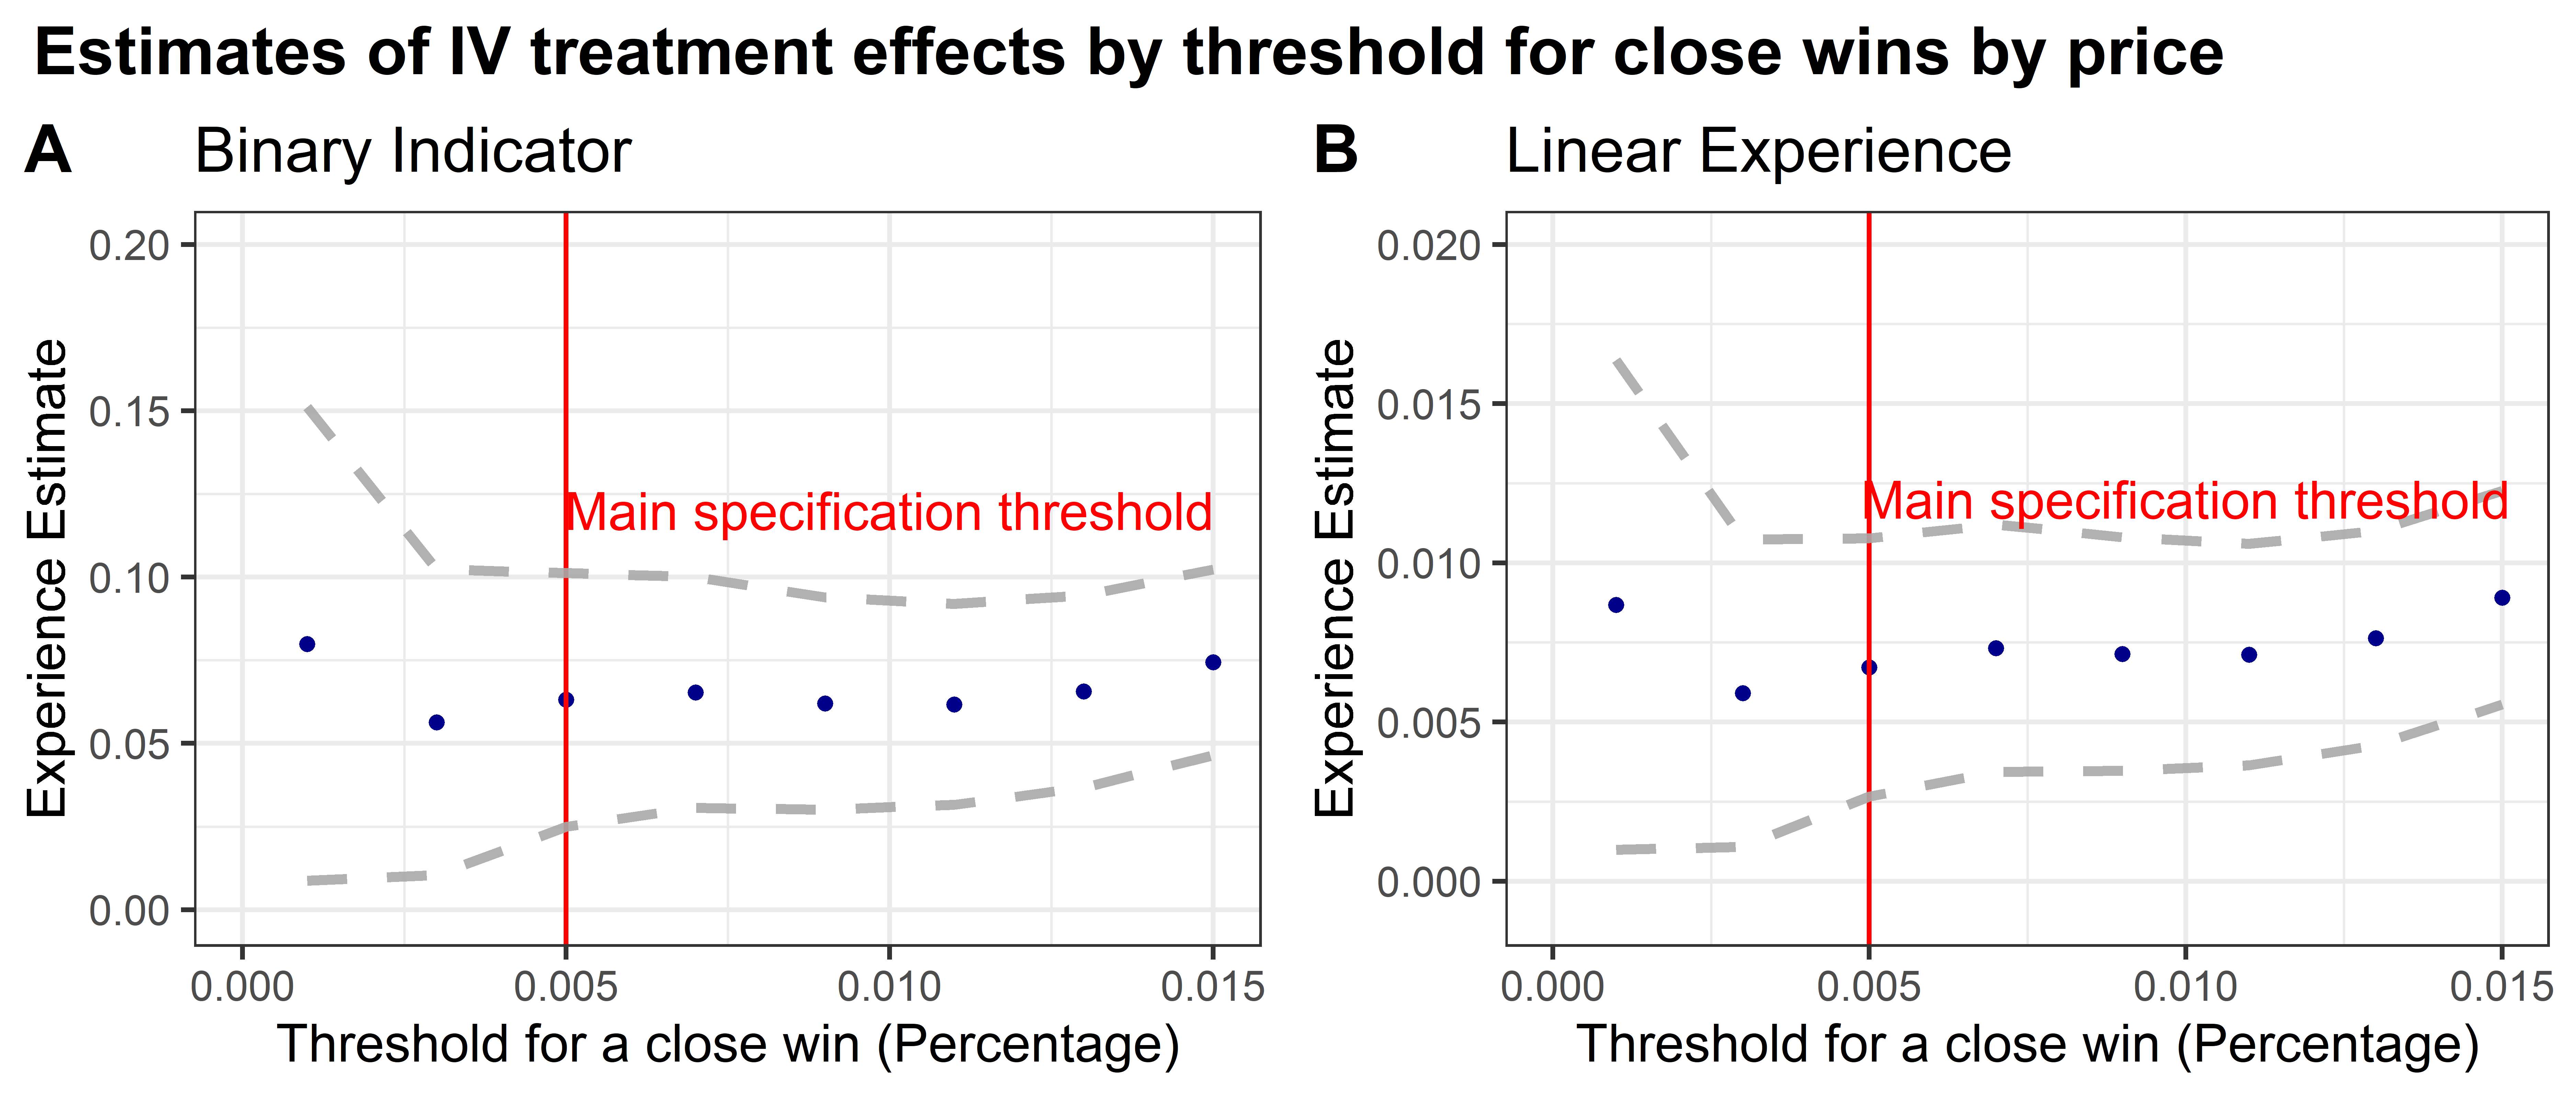
\includegraphics[scale=0.85]{robustness_threshold.png}
         \caption{Robustness analysis for threshold of close wins}
         \label{fig:close_wins_robust}

  \vskip 0.5mm
  {\justifying\footnotesize\underline{Note:} The plot shows the coefficient on experience as in the specification of Panel (5) of table \ref{tab:table_exp_1}, that is, the dependent variable is the share of contracts won in period $t$ and the dependent variable is linear experience, i.e. number of contracts won in period $(t-1)$, instrumented with close wins in period $(t-1)$. The $x$-axis shows how the coefficient varies with the threshold for what is considered a close win.\par}


     \end{figure}

%%% This is an example first chapter.  You should put chapter/appendix that you
%% write into a separate file, and add a line \include{yourfilename} to
%% main.tex, where `yourfilename.tex' is the name of the chapter/appendix file.
%% You can process specific files by typing their names in at the
%% \files=
%% prompt when you run the file main.tex through LaTeX.
\chapter{Institutional context}
\section{Procurement and Public purchases in Chile}
\subsection{Public purchases via open call for proposals}
In general, all government units employ open calls for proposals to procure differentiated and non-standard goods and services (vey undifferentiated products, like office materials, are sometimes instead developed by a different type of method called framework agreement).  Government units usually advertise the project with a public announcement in the procuring platform, receive tenders by interested firms and then award the project by ranking proposals with a weighted scoring method. In what follows we describe the auctioning process, awarding methods, some exceptions to the general rule, and legal requirements for contractors to participate in the market.

Usually, auctions have the following stages. First, the government sets up an open call for proposals for a specific project in a digital platform called Mercado Público, making available relevant documents about the requirements for the project and detailing the awarding criteria that will be employed to score proposals. Firms submit their tenders through the same digital platform, but cannot see tenders submitted by other firms. During the open call phase, firms can submit questions to the government, which, along with the government answer, are published online. When the tendering period ends, the revision of proposals is done in two steps. First, government officials examine all proposals and ensure that they fulfill the minimum formal requirements to be evaluated on an equal footing with other proposals. All the proposals that fulfill the formal requirements are considered “Accepted”. The second step is to score all the “Accepted” proposals in terms of the awarding criteria and rank them. The top proposal (or proposals, in case of multi-product auctions) is selected and awarded the project or service.

For each project the government chooses a set of items in which proposals will be evaluated on and a corresponding weight, which sum up to 100\%. The most frequent awarding items include price, technical specifications, quality, experience, etc. At the second awarding sub-stage, each proposal is given a given a score on each item,  based on rules specified in the tendering documents. Individual item's scores and multiplied by the corresponding weight and then summed up. The proposal's score is this weighted sum.

Before the call for proposals, the auctioneer must establish an estimate of the total cost of the project. If the winning proposals are above 30\% of this estimate, the government unit must justify thoroughly the reasons that justify this disparity and keep additional information of the contract for further revisions.

The buying government unit can employ two alternative procurement methods to an open call for proposals. It can develop a private auction (where only a subset of contractors are invited to submit proposals) or award directly the project to a contractor of its choice. However, there are several legal requirements for a project to be eligible for these types of procurement methods. Examples of situations where direct or private auctioning is permitted are when a very specific product is required (so there is only one or a few providers) or the project is an extreme region, where there are too few providers. These type of awarding method usually receives more scrutiny from the Contraloria, the government unit which checks if government actions are carried out within the appropriate legal rules, so they cannot be used indiscriminately.

All companies must register as public contractors in order to bid for public projects in a registry called Mercado Público. The purpose of this registry is to ensure that contractors are in good legal standing, and that they have no outstanding debts with the government treasury. It also allows to keep a track record for every contractor of past performance in government contracting. The registry is also useful to identify potential conflicts of interest between firms' executives or firms' owners with government officials, as firms must disclose their ownership scheme at the time of registering. Even though every contractor must fulfill the same minimum requirements in this registry, some government units, like the Ministry of Housing, maintain additional registers focused on the specific projects that the unit develops. These registries usually include additional requirements from firms and classify contractors into categories according to their expertise and financial capacity.
%These are discussed in the detailed section about types of projects.

\subsection{Procurement And Information}
In Chile, as a general rule all government bodies must develop procurement procedures through a digital platform called the Mercado Público (\textit{Public Market}).  This obligation was introduced by the Public Purchases Law N° 19.886 (2010) and requires from government units to develop all stages of the process only through the platforms established by the Directorate of Public Purchases, more commonly known as Chile Compra, dependent from the Ministry of Treasury.

While in the public construction sector different types of projects have different rules for how to conduct the details of the procurement process, the law mentioned above still requires from every government unit developing purchases to publish a common set of information to the digital platform. Some exceptions apply: contracts subject to considerations of national security, cases where providers cannot use the digital systems, and other considerations of major force. Among the information that the law requires to publish is the date of the auctions, any modifications to the blueprints, and the awarding decision.

The data of projects developed via Mercado Público has been made public through an open data platform, which is the primary source of our data.

%Usually, procurement can proceed through framework arrangements or project-specific auctions Framework arrangements are auctions held by the government ex-ante where firms compete to be included in menu of similar products, usually with low to medium degrees of differentiation. If they win, their product can be directly bought by a government unit without the need for a separate auction. The framework agreements are usually employed to procure simple, less-differentiated products such as office materials, notebooks, etc. In the current work, we do not include data of products bough in this way in our analysis because we are not interested in materials or standard services but rather in full construction projects.

\section{Procurement of Construction Projects}
The law 19,886 and its procedures for procurement, detailed in the previous section, regulates public purchases in general. However, it excludes from its application contracts of public works. A portion of the contracts found in our dataset fall into this definition \footnote{Not all construction works are considered public works}. In this section, we briefly detail what commonly distinguishes construction procurement from regular government purchases, what are the common features among construction procurement regulation, and what are the differences among them.

Requirements for contractors are usually increased in construction contracts to mitigate the possibility of adverse selection. We note two factors that increase requirements for firms in construction projects. First, capital availability requirements, as many units include in the awarding criteria measures of equity to reduce the probability of contractor bankruptcy or loss of access to credit during the project. Second, many construction projects require a bond that can be between 3-10\% of the total value of the project from the contractor to insure against problems during the delivery phase.

Among construction projects with different types of applicable regulation, we usually see as common features of the procurement and awarding process a competitive call for proposals and a two stage awarding process. The first stage examines formal and technical requirements and the second assigns scores in the awarding criteria of the project. Differences among construction projects' regulation relate to the requirements for contractors to participate in auctions, the types of criteria that can be used to award the project, and the degree of discretion that can be employed in the process in general. Increased levels of contractor requirement or less discretionary processes are usually linked to more complex or bigger projects. For example, most projects form the Ministry of Housing requires prequalification steps and registering in a unit-specific registry which ensures financial capacity, experience, and skills.

Finally, even if a contract has its own particular set of applicable regulations, the Law of Public Purchases states that its own set own set of regulations shall be applicable wherever it is not contradictory with the more specific regulation.

The appendix \ref{section:app_inst} shows further disaggregation into the types of projects in the dataset and the applicable regulation to each of them, which was too long to place here.
%Altough the construction projects in our dataset are construction contracts, only a portion of them fall under the category of public works and would thus be excluded from its application.

%We now describe the particularities of the institutional framework for the procurement of construction projects. First, we advance some common qualitative differences, and given the heterogeneity of the projects in the dataset we next detail the relevant context for each type of project available in it.


%We end up detailing projects not found in the dataset.

%For example, in the case of hospitals, the Ministry of  Health is in charge of defining the projects, technical requirements, etc. of the hospitals that will be built. However, it usually signs agreements with the Ministry of Public Works where the Ministry of Public Works either i) directly oversees the auction and execution of the project via the Architecture Directorate or ii) develops a Public-Private Partnership to award to a contractor that will design, build, and operate the project. The last of these agreements was done in 2018 and it specified that 7 hospitals would be directly overseen by the Architectural Directorate and 18 would be developed via PPPs.

%The first way is to directly procure smaller projects (repairments, small building works, etc.) with no support. This is mostly employed by municipalities developing small urban projects, or by other government units developing small repair and maintenance projects. These types of projects fall directly under the regulations of the 19.86 law and the specific regulations of each procuring body.

%Some construction projects is that they require from contractors to be registered in a special Registry, which has specific experience, capital, and other requirements. Two of the government units that employ this special registry is the Ministry of Housing and the Ministry of Public Works.

%Although the previous elements describe some qualitative differences commonly found, project institutional context can differ highly depending on the specific type of the project. The following section details the different types of projects found in the dataset and their main institutional frameworks.
%The importance of considering the particularities of the construction sector is that several of the specific arrangements for these projects imply higher entry barriers to new contractors, which effect could be added to an eventual effect of experience on outcomes, which is the focus of the investigation.

%In some types of projects, for example, urban road projects, municipalities usually associate with the Ministry of Housing and Urbanism (MINVU) for financial or technical support. In rural areas, urban works developed by the Municipality include sewer and potable water infrastructure, in which they are supported by the Ministry of Public Works (MOP) or MINVU. In all these cases, the relevant legal framework will have additional requirements.
%\subsection{Summary}
%Projects in our investigation have different types of regulations applicable to them depending on the type, scope and size of the project. In general, we find the following common feature in the procurement process: an open call for proposals, a two stage awarding process, where the first stage examines formal and technical requirements and the second assigns scores in the awarding criteria of the project.With respect to other public purchases, requirements for contractors are usually increased in construction contracts to mitigate the possibility of adverse selection. We note two factors that increase requirements for firms in construction projects. First, capital avalaibility requirements, as many units include in the awarding criteria measures of patrimonio to reduce the probability fof bankruptcy or no access to credit during the project. Second, surety bonds, as many construction projects require a bond that can be between 3-10\% of the total value of the project from the contractor to insure against problems during delivery.Differences among construction projects' frameworks relate to the requirements to contractors to participate in auctions. More complex and certain types of projects requires prequalification steps and registering in a unit specific- which ensures financial capacity, experience, and skills.

%Finally, even if a contract has its own set of applicable regulation, the Law of Public Purchases states that in everything that is not explicititly changed in the specific regulation, it shall be applicable.

%include{chapData}
%\appendix
%\chapter{Tables}

\begin{table}
\caption{Armadillos}
\label{arm:table}
\begin{center}
\begin{tabular}{||l|l||}\hline
Armadillos & are \\\hline
our	   & friends \\\hline
\end{tabular}
\end{center}
\end{table}

\clearpage
\newpage

%\chapter{Figures}

\vspace*{-3in}

\begin{figure}
\vspace{2.4in}
\caption{Armadillo slaying lawyer.}
\label{arm:fig1}
\end{figure}
\clearpage
\newpage

\begin{figure}
\vspace{2.4in}
\caption{Armadillo eradicating national debt.}
\label{arm:fig2}
\end{figure}
\clearpage
\newpage

%%% This defines the bibliography file (main.bib) and the bibliography style.
%% If you want to create a bibliography file by hand, change the contents of
%% this file to a `thebibliography' environment.  For more information 
%% see section 4.3 of the LaTeX manual.
\begin{singlespace}
\bibliography{main}
\bibliographystyle{plain}
\end{singlespace}

\end{document}
